\documentclass[]{article}
\usepackage[T1]{fontenc}
\usepackage{lmodern}
\usepackage{amssymb,amsmath}
\usepackage{ifxetex,ifluatex}
\usepackage{fixltx2e} % provides \textsubscript
\usepackage{endfloat}

% use upquote if available, for straight quotes in verbatim environments
\IfFileExists{upquote.sty}{\usepackage{upquote}}{}
\ifnum 0\ifxetex 1\fi\ifluatex 1\fi=0 % if pdftex
  \usepackage[utf8]{inputenc}
\else % if luatex or xelatex
  \ifxetex
    \usepackage{mathspec}
    \usepackage{xltxtra,xunicode}
  \else
    \usepackage{fontspec}
  \fi
  \defaultfontfeatures{Mapping=tex-text,Scale=MatchLowercase}
  \newcommand{\euro}{€}
\fi
% use microtype if available
\IfFileExists{microtype.sty}{\usepackage{microtype}}{}
\usepackage{color}
\usepackage{fancyvrb}
\newcommand{\VerbBar}{|}
\newcommand{\VERB}{\Verb[commandchars=\\\{\}]}
\DefineVerbatimEnvironment{Highlighting}{Verbatim}{commandchars=\\\{\}}
% Add ',fontsize=\small' for more characters per line
\newenvironment{Shaded}{}{}
\newcommand{\KeywordTok}[1]{\textcolor[rgb]{0.00,0.44,0.13}{\textbf{{#1}}}}
\newcommand{\DataTypeTok}[1]{\textcolor[rgb]{0.56,0.13,0.00}{{#1}}}
\newcommand{\DecValTok}[1]{\textcolor[rgb]{0.25,0.63,0.44}{{#1}}}
\newcommand{\BaseNTok}[1]{\textcolor[rgb]{0.25,0.63,0.44}{{#1}}}
\newcommand{\FloatTok}[1]{\textcolor[rgb]{0.25,0.63,0.44}{{#1}}}
\newcommand{\CharTok}[1]{\textcolor[rgb]{0.25,0.44,0.63}{{#1}}}
\newcommand{\StringTok}[1]{\textcolor[rgb]{0.25,0.44,0.63}{{#1}}}
\newcommand{\CommentTok}[1]{\textcolor[rgb]{0.38,0.63,0.69}{\textit{{#1}}}}
\newcommand{\OtherTok}[1]{\textcolor[rgb]{0.00,0.44,0.13}{{#1}}}
\newcommand{\AlertTok}[1]{\textcolor[rgb]{1.00,0.00,0.00}{\textbf{{#1}}}}
\newcommand{\FunctionTok}[1]{\textcolor[rgb]{0.02,0.16,0.49}{{#1}}}
\newcommand{\RegionMarkerTok}[1]{{#1}}
\newcommand{\ErrorTok}[1]{\textcolor[rgb]{1.00,0.00,0.00}{\textbf{{#1}}}}
\newcommand{\NormalTok}[1]{{#1}}
\usepackage{graphicx}
% Redefine \includegraphics so that, unless explicit options are
% given, the image width will not exceed the width of the page.
% Images get their normal width if they fit onto the page, but
% are scaled down if they would overflow the margins.
\makeatletter
\def\ScaleIfNeeded{%
  \ifdim\Gin@nat@width>\linewidth
    \linewidth
  \else
    \Gin@nat@width
  \fi
}
\makeatother
\let\Oldincludegraphics\includegraphics
{%
 \catcode`\@=11\relax%
 \gdef\includegraphics{\@ifnextchar[{\Oldincludegraphics}{\Oldincludegraphics[width=\ScaleIfNeeded]}}%
}%
\ifxetex
  \usepackage[setpagesize=false, % page size defined by xetex
              unicode=false, % unicode breaks when used with xetex
              xetex]{hyperref}
\else
  \usepackage[unicode=true]{hyperref}
\fi
\hypersetup{breaklinks=true,
            bookmarks=true,
            pdfauthor={Karl Benedict; Director, Earth Data Analysis Center; Associate Professor, College of University Libraries & Learning Sciences; University of New Mexico; kbene@unm.edu},
            pdftitle={The Google Maps API and OpenLayers Javascript Framework: a NMGIC Workshop},
            colorlinks=true,
            citecolor=blue,
            urlcolor=blue,
            linkcolor=magenta,
            pdfborder={0 0 0}}
\urlstyle{same}  % don't use monospace font for urls
\setlength{\parindent}{0pt}
\setlength{\parskip}{6pt plus 2pt minus 1pt}
\setlength{\emergencystretch}{3em}  % prevent overfull lines

\oddsidemargin = 0pt
\topmargin = -36pt
\textwidth = 468pt
\textheight = 648pt

\setcounter{secnumdepth}{0}

\title{The Google Maps API and OpenLayers Javascript Framework: a NMGIC
Workshop}
\author{\textbf{Karl Benedict} \and Director, Earth Data Analysis Center \and Associate Professor, College of University Libraries \& Learning
Sciences \and \emph{University of New Mexico} \and kbene@unm.edu}
\date{May 1, 2014}

\begin{document}
\maketitle

{
\hypersetup{linkcolor=black}
\setcounter{tocdepth}{3}
\tableofcontents
}
\section{Overview}\label{overview}

\subsubsection{Presentation Copy Links}\label{presentation-copy-links}

\begin{itemize}
\itemsep1pt\parskip0pt\parsep0pt
\item
  HTML Version:
  \url{http://karlbenedict.com/presentations/2014-04-NMGIC}
\item
  PDF Version:
  \url{http://karlbenedict.com/presentations/2014-04-NMGIC/presentation.md.pdf}
\item
  Example files (GitHub): \url{http://tinyurl.com/lm3almv}
\end{itemize}

\section{Google Maps API}\label{google-maps-api}

\subsection{Introduction}\label{introduction}

\subsubsection{Outline}\label{outline}

\begin{itemize}
\itemsep1pt\parskip0pt\parsep0pt
\item
  What is an API
\item
  The Google Maps API

  \begin{itemize}
  \itemsep1pt\parskip0pt\parsep0pt
  \item
    Version
  \item
    Reference Information
  \item
    Key Components
  \item
    Examples
  \end{itemize}
\end{itemize}

\subsubsection{What is an API}\label{what-is-an-api}

\begin{itemize}
\itemsep1pt\parskip0pt\parsep0pt
\item
  API Stands for Application Programming Interface
\end{itemize}

\begin{quote}
An Application Programming Interface (API) is a particular set of rules
and specifications that a software program can follow to access and make
use of the services and resources provided by another particular
software program that implements that API. It serves as an interface
between different software programs and facilitates their interaction,
similar to the way the user interface facilitates interaction between
humans and computers. -- From Wikipedia:
\url{http://en.wikipedia.org/wiki/Api}
\end{quote}

\begin{itemize}
\itemsep1pt\parskip0pt\parsep0pt
\item
  The Google Maps API provides an interface for interacting with
  Google's mapping services from external web applications
\end{itemize}

\subsubsection{Google Maps API Version}\label{google-maps-api-version}

\begin{itemize}
\itemsep1pt\parskip0pt\parsep0pt
\item
  The version of the Google Maps API used in this session is v3 of the
  Javascript API

  \begin{itemize}
  \itemsep1pt\parskip0pt\parsep0pt
  \item
    Freely usable for free applications
  \item
    Subject to Google's
    \href{https://developers.google.com/maps/terms?hl=en}{Terms of
    Service}
  \item
    No longer requires a Google API key, but one is
    \href{http://tinyurl.com/d52lcm2}{recommended for tracking usage}
  \end{itemize}
\item
  Key capabilities in v3

  \begin{itemize}
  \itemsep1pt\parskip0pt\parsep0pt
  \item
    Interactive maps based on Google's mapping engine (contrast w.
    static maps API)
  \item
    Optimized for desktop and mobile platforms and applications
  \end{itemize}
\end{itemize}

\subsubsection{Reference Information}\label{reference-information}

\begin{description}
\item[Google Maps API Family]
\url{http://code.google.com/apis/maps/}
\item[Javascript API Home Page]
\url{http://code.google.com/apis/maps/documentation/javascript/}
\item[Javascript Basics Entry Page]
\url{http://code.google.com/apis/maps/documentation/javascript/basics.html}
\item[Javascript API v3 Tutorial Page]
\url{http://code.google.com/apis/maps/documentation/javascript/tutorial.html}
\end{description}

\subsubsection{Key Components}\label{key-components}

Map \href{http://tinyurl.com/mlsj3ar}{object options}

\begin{description}
\item[Types (required)]
ROADMAP

SATELLITE

HYBRID

TERRAIN
\item[Latitude and Longitude (required)]
specification of where the map should initially be centered
\item[Zoom Level (required)]
0=global, higher values increasingly local. Limited by map type
\end{description}

\subsubsection{Controls}\label{controls}

\begin{itemize}
\itemsep1pt\parskip0pt\parsep0pt
\item
  Available Controls (enabled through map options)
  \href{http://tinyurl.com/nryup5j}{default controls}

  \begin{itemize}
  \itemsep1pt\parskip0pt\parsep0pt
  \item
    Zoom Control
  \item
    Pan Control
  \item
    Scale Control
  \item
    MapType Control
  \item
    Street View Control
  \end{itemize}
\item
  Different control styles may be defined
\item
  Controls may be positioned
  \href{http://tinyurl.com/p3hc5gk}{positioning options}
\item
  Custom controls may be defined and attached to fixed location in the
  map
\end{itemize}

\subsubsection{Overlays}\label{overlays}

Overlay Types
\href{http://code.google.com/apis/maps/documentation/javascript/overlays.html}{documentation}

\begin{description}
\item[Marker]
points depicted by specified or defined icons at locations within the
map
\item[Polyline]
linear features defined by multiple points with a defined style for the
line
\item[Polygon]
closed features defined by multiple points. Supports multi-polygons, and
donuts. Line and fill styles may be specified.
\item[(Ground) Overlay Maps]
Image-based map layers that replace or overlay Google layers -
registered to the map coordinates
\item[Info Windows]
floating content windows for displaying content defined as HTML, a DOM
element, or text string
\item[Layers]
Grouped display content assigned to a specific layer: KmlLayer,
FusionTablesLayer, TrafficLayer, BicyclingLayer
\item[Custom Overlays]
definition of programmatically controlled layers
\end{description}

\subsubsection{Services}\label{services}

\begin{itemize}
\itemsep1pt\parskip0pt\parsep0pt
\item
  Geocoding Service

  \begin{itemize}
  \itemsep1pt\parskip0pt\parsep0pt
  \item
    Forward and reverse geocoding:

    \begin{itemize}
    \itemsep1pt\parskip0pt\parsep0pt
    \item
      address to LatLon
    \item
      LatLon to Nearest Address
    \end{itemize}
  \item
    May be biased to current viewport, region
  \end{itemize}
\item
  Directions

  \begin{itemize}
  \itemsep1pt\parskip0pt\parsep0pt
  \item
    Based upon an origin, destination, and a variety of additional
    options
  \item
    Available directions and rendered route
  \end{itemize}
\item
  Elevation

  \begin{itemize}
  \itemsep1pt\parskip0pt\parsep0pt
  \item
    Delivery of elevation data for locations or paths
  \end{itemize}
\item
  Streetview

  \begin{itemize}
  \itemsep1pt\parskip0pt\parsep0pt
  \item
    Integration of Google Streetview within a DOM element
  \end{itemize}
\item
  Maximum Zoom

  \begin{itemize}
  \itemsep1pt\parskip0pt\parsep0pt
  \item
    Provides information about the maximum available zoom level
  \end{itemize}
\end{itemize}

\subsubsection{Events}\label{events}

\begin{itemize}
\itemsep1pt\parskip0pt\parsep0pt
\item
  Events provide the ability to attach custom behaviors to events in the
  interface. For example:

  \begin{itemize}
  \itemsep1pt\parskip0pt\parsep0pt
  \item
    Changing items in the interface as the user zooms in on a map
  \item
    Displaying additional information outside the map when the user
    clicks a location in the map
  \item
    Synchronizing the behavior of multiple maps as the user interacts
    with one map
  \end{itemize}
\item
  Requires higher-level Javascript that we will cover here
\end{itemize}

\subsection{Examples}\label{examples}

\subsubsection{Simple - Roadmap}\label{simple---roadmap}

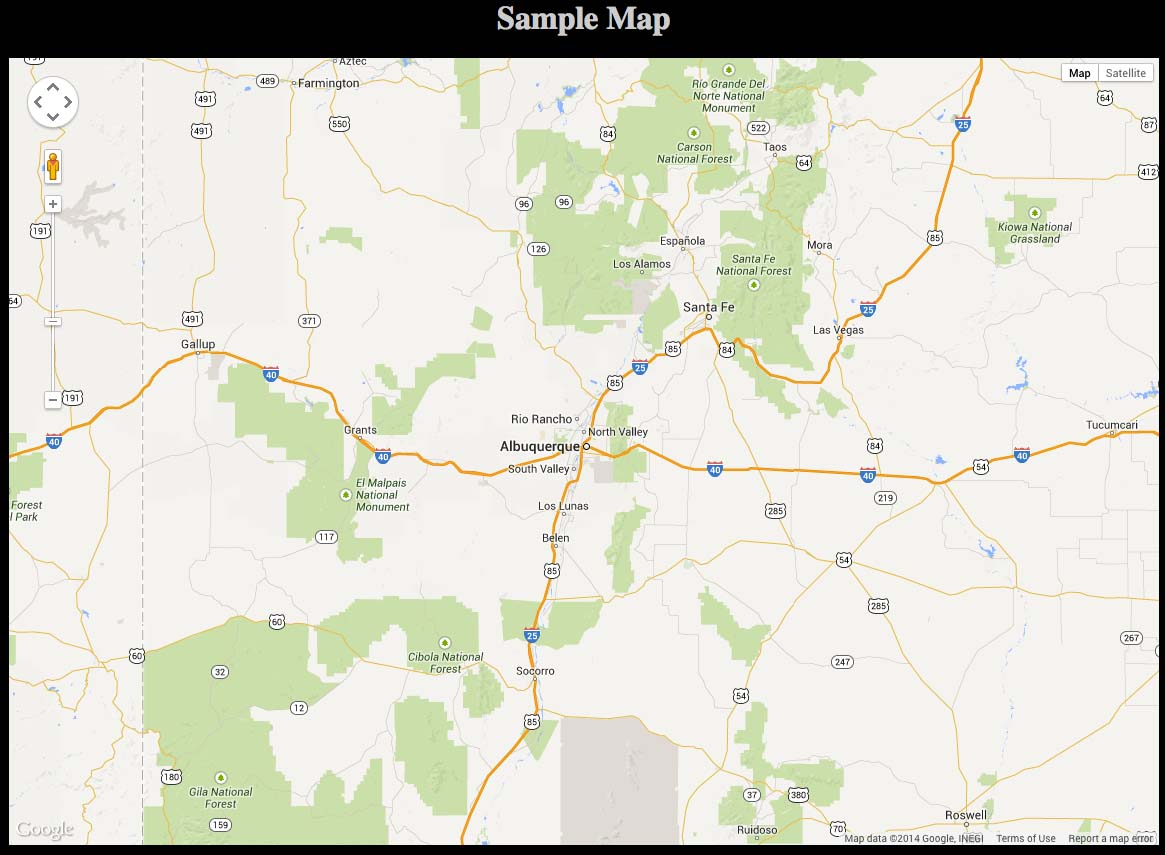
\includegraphics{images/google_01.jpg}~

\url{http://karlbenedict.com/presentations/2014-04-NMGIC/examples/gmaps01.html}

\hyperdef{}{roadmap}{\label{roadmap}}
\begin{Shaded}
\begin{Highlighting}[numbers=left,,]
\DataTypeTok{<!DOCTYPE }\NormalTok{html}\DataTypeTok{>}
\KeywordTok{<html>}
    \KeywordTok{<head>}
        \KeywordTok{<style}\OtherTok{ type=}\StringTok{"text/css"}\KeywordTok{>}
            \NormalTok{html }\KeywordTok{\{} \KeywordTok{height:} \DataTypeTok{100%} \KeywordTok{\}}
            \NormalTok{body }\KeywordTok{\{} \KeywordTok{height:} \DataTypeTok{100%}\KeywordTok{;} 
                \KeywordTok{margin:} \DataTypeTok{0px}\KeywordTok{;} 
                \KeywordTok{padding:} \DataTypeTok{0px}\KeywordTok{;} 
                \KeywordTok{background-color:} \DataTypeTok{black}\KeywordTok{;} 
                \KeywordTok{color:} \DataTypeTok{#CCCCCC}\KeywordTok{;}
                \KeywordTok{text-align:} \DataTypeTok{center}\KeywordTok{\}}
            \FloatTok{#map_canvas} \KeywordTok{\{} \KeywordTok{width:}\DataTypeTok{90%}\KeywordTok{;} 
                \KeywordTok{height:}\DataTypeTok{80%}\KeywordTok{;} 
                \KeywordTok{margin-left:}\DataTypeTok{auto}\KeywordTok{;} 
                \KeywordTok{margin-right:} \DataTypeTok{auto} \KeywordTok{\}}
        \KeywordTok{</style>}
        \KeywordTok{<script}\OtherTok{ type=}\StringTok{"text/javascript"}
\OtherTok{            src=}\StringTok{"http://maps.google.com/maps/api/js?sensor=false"}\KeywordTok{>}
        \KeywordTok{</script>}
        \KeywordTok{<script}\OtherTok{ type=}\StringTok{"text/javascript"}\KeywordTok{>}
\ErrorTok{            function initialize() \{}
\ErrorTok{            var classroom = new google.maps.LatLng(35.084280,-106.624073)}
            \KeywordTok{var} \NormalTok{myOptions = \{}
                \DataTypeTok{zoom}\NormalTok{: }\DecValTok{8}\NormalTok{,}
                \DataTypeTok{center}\NormalTok{: classroom,}
                \DataTypeTok{mapTypeId}\NormalTok{: }\OtherTok{google}\NormalTok{.}\OtherTok{maps}\NormalTok{.}\OtherTok{MapTypeId}\NormalTok{.}\FunctionTok{ROADMAP}
            \NormalTok{\};}
\ErrorTok{            var map = new google.maps.Map(}
\ErrorTok{                document.getElementById("map_canvas"),}
                \NormalTok{myOptions);}
            \NormalTok{\}}
        \KeywordTok{</script>}
    \KeywordTok{</head>}

    \KeywordTok{<body}\OtherTok{ onload=}\StringTok{"initialize()"}\KeywordTok{>}
        \KeywordTok{<h1>}\NormalTok{Sample Map}\KeywordTok{</h1>}
        \KeywordTok{<div}\OtherTok{ id=}\StringTok{"map_canvas"}\KeywordTok{></div>}
    \KeywordTok{</body>}
\KeywordTok{</html>}
\end{Highlighting}
\end{Shaded}

\subsubsection{Simple - Satellite}\label{simple---satellite}

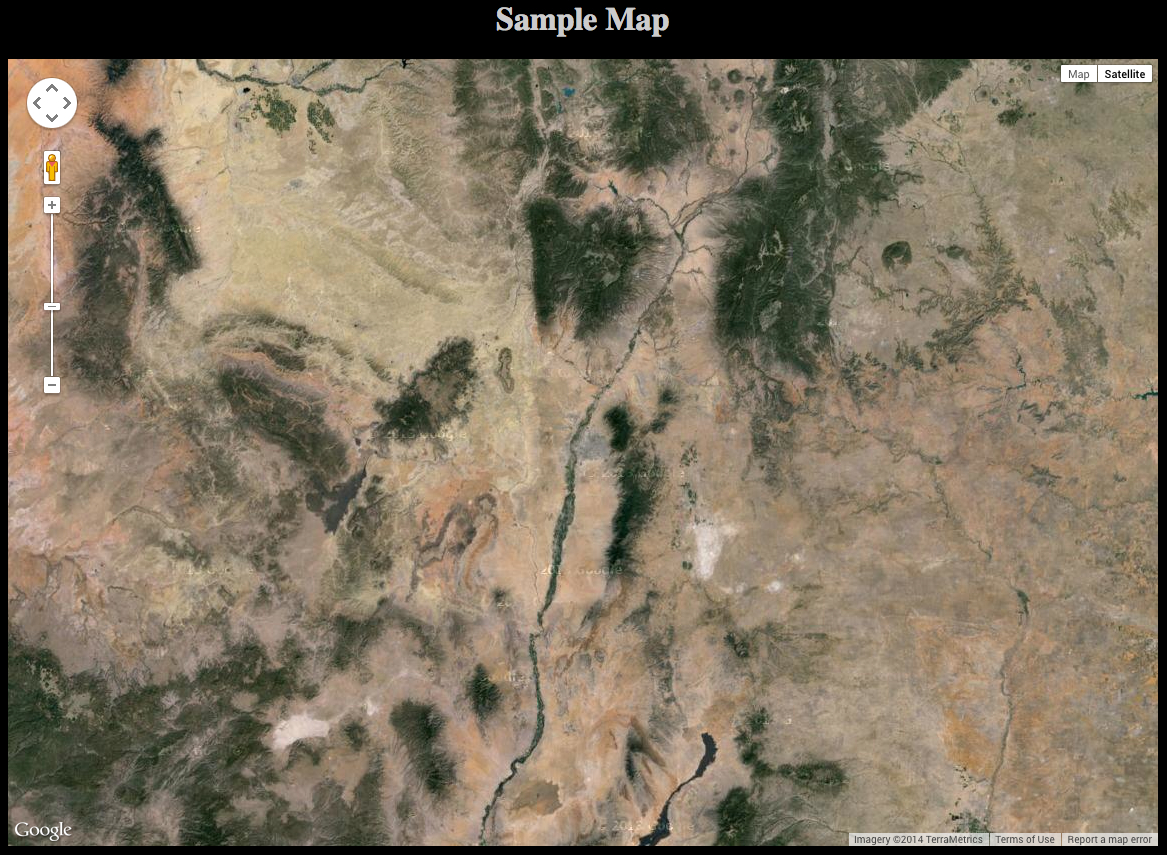
\includegraphics{images/google_02.jpg}~

\url{http://karlbenedict.com/presentations/2014-04-NMGIC/examples/gmaps02.html}

\hyperdef{}{satellite}{\label{satellite}}
\begin{Shaded}
\begin{Highlighting}[numbers=left,,]
\DataTypeTok{<!DOCTYPE }\NormalTok{html}\DataTypeTok{>}

\KeywordTok{<html>}
    \KeywordTok{<head>}
        \KeywordTok{<style}\OtherTok{ type=}\StringTok{"text/css"}\KeywordTok{>}
            \NormalTok{html }\KeywordTok{\{} \KeywordTok{height:} \DataTypeTok{100%} \KeywordTok{\}}
            \NormalTok{body }\KeywordTok{\{} \KeywordTok{height:} \DataTypeTok{100%}\KeywordTok{;} 
                \KeywordTok{margin:} \DataTypeTok{0px}\KeywordTok{;} 
                \KeywordTok{padding:} \DataTypeTok{0px}\KeywordTok{;} 
                \KeywordTok{background-color:} \DataTypeTok{black}\KeywordTok{;} 
                \KeywordTok{color:} \DataTypeTok{#CCCCCC}\KeywordTok{;}
                \KeywordTok{text-align:} \DataTypeTok{center}\KeywordTok{\}}
            \FloatTok{#map_canvas} \KeywordTok{\{} \KeywordTok{width:}\DataTypeTok{90%}\KeywordTok{;} 
                \KeywordTok{height:}\DataTypeTok{80%}\KeywordTok{;} 
                \KeywordTok{margin-left:} \DataTypeTok{auto}\KeywordTok{;} 
                \KeywordTok{margin-right:} \DataTypeTok{auto} \KeywordTok{\}}
        \KeywordTok{</style>}
        \KeywordTok{<script}\OtherTok{ type=}\StringTok{"text/javascript"}
\OtherTok{            src=}\StringTok{"http://maps.google.com/maps/api/js?sensor=false"}\KeywordTok{>}
        \KeywordTok{</script>}
        \KeywordTok{<script}\OtherTok{ type=}\StringTok{"text/javascript"}\KeywordTok{>}
\ErrorTok{            function initialize() \{}
\ErrorTok{                var classroom = new google.maps.LatLng(35.084280,-106.624073)}
                \KeywordTok{var} \NormalTok{myOptions = \{}
                    \DataTypeTok{zoom}\NormalTok{: }\DecValTok{8}\NormalTok{,}
                    \DataTypeTok{center}\NormalTok{: classroom,}
                    \DataTypeTok{mapTypeId}\NormalTok{: }\OtherTok{google}\NormalTok{.}\OtherTok{maps}\NormalTok{.}\OtherTok{MapTypeId}\NormalTok{.}\FunctionTok{SATELLITE}
                \NormalTok{\};}
\ErrorTok{                var map = new google.maps.Map(}
\ErrorTok{                    document.getElementById("map_canvas"), }
                    \NormalTok{myOptions);}
            \NormalTok{\}}
        \KeywordTok{</script>}
    \KeywordTok{</head>}
    
    \KeywordTok{<body}\OtherTok{ onload=}\StringTok{"initialize()"}\KeywordTok{>}
        \KeywordTok{<h1>}\NormalTok{Sample Map}\KeywordTok{</h1>}
        \KeywordTok{<div}\OtherTok{ id=}\StringTok{"map_canvas"}\KeywordTok{></div>}
    \KeywordTok{</body>}
\KeywordTok{</html>}
\end{Highlighting}
\end{Shaded}

\subsubsection{Simple - Hybrid}\label{simple---hybrid}

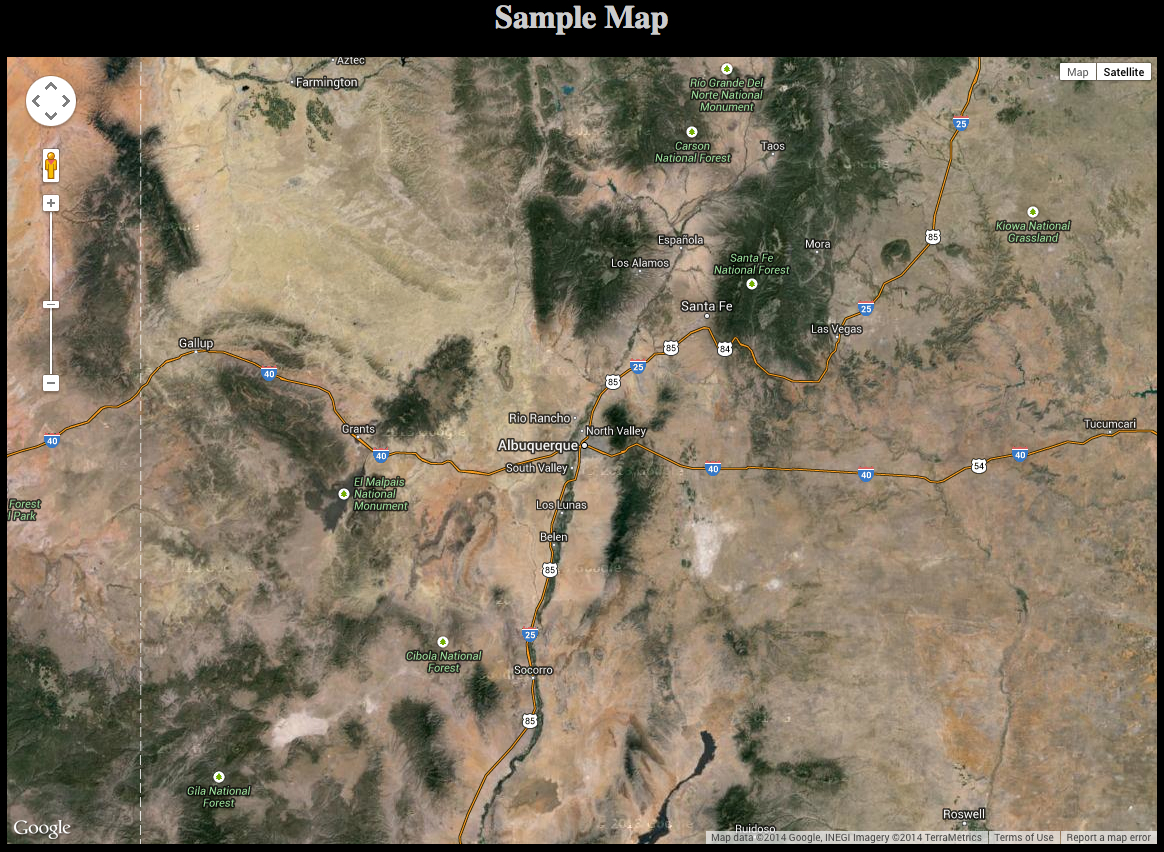
\includegraphics{images/google_03.jpg}~

\url{http://karlbenedict.com/presentations/2014-04-NMGIC/examples/gmaps03.html}

\hyperdef{}{hybrid}{\label{hybrid}}
\begin{Shaded}
\begin{Highlighting}[numbers=left,,]
\DataTypeTok{<!DOCTYPE }\NormalTok{html}\DataTypeTok{>}
\KeywordTok{<html>}
    \KeywordTok{<head>}
        \KeywordTok{<style}\OtherTok{ type=}\StringTok{"text/css"}\KeywordTok{>}
          \NormalTok{html }\KeywordTok{\{} \KeywordTok{height:} \DataTypeTok{100%} \KeywordTok{\}}
          \NormalTok{body }\KeywordTok{\{} \KeywordTok{height:} \DataTypeTok{100%}\KeywordTok{;} 
            \KeywordTok{margin:} \DataTypeTok{0px}\KeywordTok{;} 
            \KeywordTok{padding:} \DataTypeTok{0px}\KeywordTok{;} 
            \KeywordTok{background-color:} \DataTypeTok{black}\KeywordTok{;} 
            \KeywordTok{color:} \DataTypeTok{#CCCCCC}\KeywordTok{;}
            \KeywordTok{text-align:} \DataTypeTok{center}\KeywordTok{\}}
          \FloatTok{#map_canvas} \KeywordTok{\{} \KeywordTok{width:}\DataTypeTok{90%}\KeywordTok{;} 
            \KeywordTok{height:}\DataTypeTok{80%}\KeywordTok{;} 
            \KeywordTok{margin-left:} \DataTypeTok{auto}\KeywordTok{;} 
            \KeywordTok{margin-right:} \DataTypeTok{auto} \KeywordTok{\}}
        \KeywordTok{</style>}
        \KeywordTok{<script}\OtherTok{ type=}\StringTok{"text/javascript"}
\OtherTok{            src=}\StringTok{"http://maps.google.com/maps/api/js?sensor=false"}\KeywordTok{>}
        \KeywordTok{</script>}
        \KeywordTok{<script}\OtherTok{ type=}\StringTok{"text/javascript"}\KeywordTok{>}
\ErrorTok{          function initialize() \{}
\ErrorTok{            var classroom = new google.maps.LatLng(35.084280,-106.624073)}
            \KeywordTok{var} \NormalTok{myOptions = \{}
              \DataTypeTok{zoom}\NormalTok{: }\DecValTok{8}\NormalTok{,}
              \DataTypeTok{center}\NormalTok{: classroom,}
              \DataTypeTok{mapTypeId}\NormalTok{: }\OtherTok{google}\NormalTok{.}\OtherTok{maps}\NormalTok{.}\OtherTok{MapTypeId}\NormalTok{.}\FunctionTok{HYBRID}
            \NormalTok{\};}
\ErrorTok{            var map = new google.maps.Map(}
\ErrorTok{                document.getElementById("map_canvas"),}
                \NormalTok{myOptions);}
          \NormalTok{\}}
        \KeywordTok{</script>}
    \KeywordTok{</head>}
    
    \KeywordTok{<body}\OtherTok{ onload=}\StringTok{"initialize()"}\KeywordTok{>}
      \KeywordTok{<h1>}\NormalTok{Sample Map}\KeywordTok{</h1>}
      \KeywordTok{<div}\OtherTok{ id=}\StringTok{"map_canvas"}\KeywordTok{></div>}
    \KeywordTok{</body>}

\KeywordTok{</html>}
\end{Highlighting}
\end{Shaded}

\subsubsection{Simple - Terrain}\label{simple---terrain}

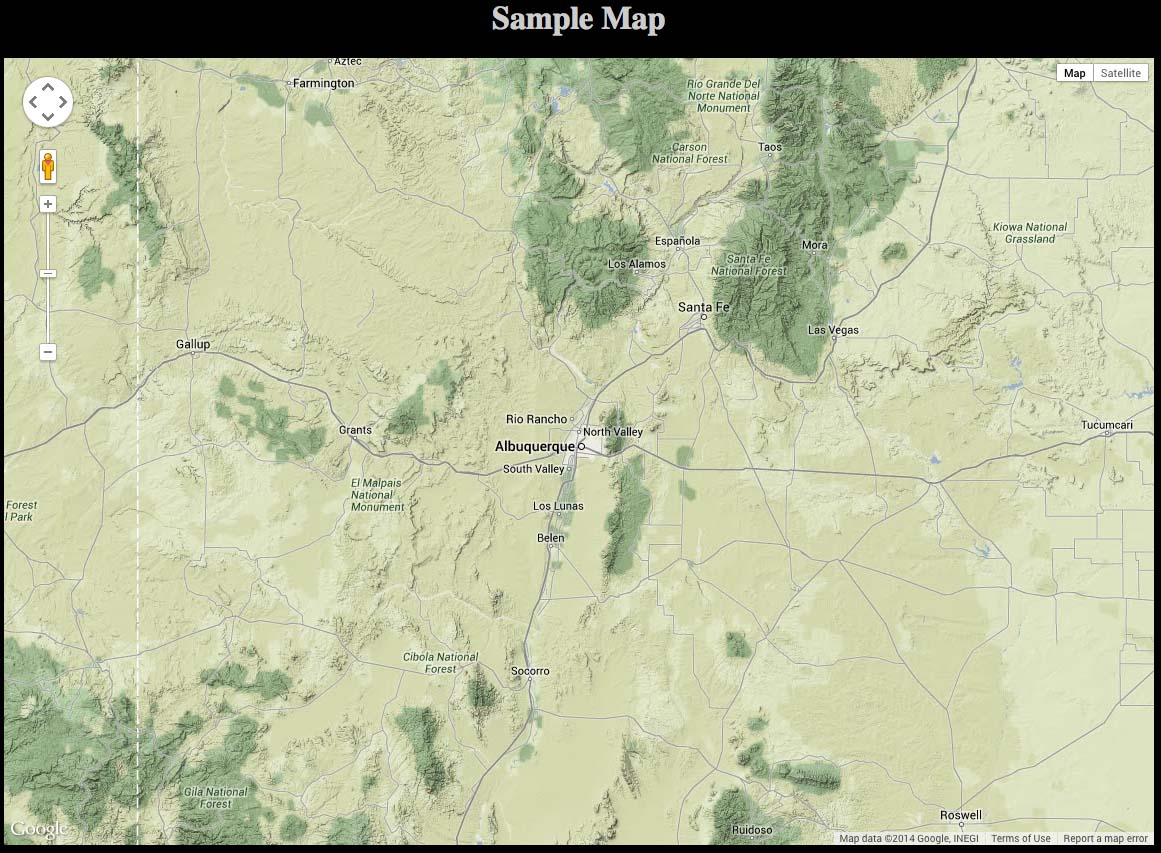
\includegraphics{images/google_04.jpg}~

\url{http://karlbenedict.com/presentations/2014-04-NMGIC/examples/gmaps04.html}

\hyperdef{}{terrain}{\label{terrain}}
\begin{Shaded}
\begin{Highlighting}[numbers=left,,]
\DataTypeTok{<!DOCTYPE }\NormalTok{html}\DataTypeTok{>}
\KeywordTok{<html>}
    \KeywordTok{<head>}
        \KeywordTok{<style}\OtherTok{ type=}\StringTok{"text/css"}\KeywordTok{>}
          \NormalTok{html }\KeywordTok{\{} \KeywordTok{height:} \DataTypeTok{100%} \KeywordTok{\}}
          \NormalTok{body }\KeywordTok{\{} \KeywordTok{height:} \DataTypeTok{100%}\KeywordTok{;} 
            \KeywordTok{margin:} \DataTypeTok{0px}\KeywordTok{;} 
            \KeywordTok{padding:} \DataTypeTok{0px}\KeywordTok{;} 
            \KeywordTok{background-color:} \DataTypeTok{black}\KeywordTok{;} 
            \KeywordTok{color:} \DataTypeTok{#CCCCCC}\KeywordTok{;}
            \KeywordTok{text-align:} \DataTypeTok{center}\KeywordTok{\}}
          \FloatTok{#map_canvas} \KeywordTok{\{} \KeywordTok{width:}\DataTypeTok{90%}\KeywordTok{;} 
            \KeywordTok{height:}\DataTypeTok{80%}\KeywordTok{;} 
            \KeywordTok{margin-left:} \DataTypeTok{auto}\KeywordTok{;} 
            \KeywordTok{margin-right:} \DataTypeTok{auto} \KeywordTok{\}}
        \KeywordTok{</style>}
        \KeywordTok{<script}\OtherTok{ type=}\StringTok{"text/javascript"}
\OtherTok{            src=}\StringTok{"http://maps.google.com/maps/api/js?sensor=false"}\KeywordTok{>}
        \KeywordTok{</script>}
        \KeywordTok{<script}\OtherTok{ type=}\StringTok{"text/javascript"}\KeywordTok{>}
\ErrorTok{          function initialize() \{}
\ErrorTok{            var classroom = new google.maps.LatLng(35.084280,-106.624073)}
            \KeywordTok{var} \NormalTok{myOptions = \{}
              \DataTypeTok{zoom}\NormalTok{: }\DecValTok{8}\NormalTok{,}
              \DataTypeTok{center}\NormalTok{: classroom,}
              \DataTypeTok{mapTypeId}\NormalTok{: }\OtherTok{google}\NormalTok{.}\OtherTok{maps}\NormalTok{.}\OtherTok{MapTypeId}\NormalTok{.}\FunctionTok{TERRAIN}
            \NormalTok{\};}
\ErrorTok{            var map = new google.maps.Map(}
\ErrorTok{                document.getElementById("map_canvas"),}
                \NormalTok{myOptions);}
          \NormalTok{\}}
        \KeywordTok{</script>}
    \KeywordTok{</head>}
    
    \KeywordTok{<body}\OtherTok{ onload=}\StringTok{"initialize()"}\KeywordTok{>}
      \KeywordTok{<h1>}\NormalTok{Sample Map}\KeywordTok{</h1>}
      \KeywordTok{<div}\OtherTok{ id=}\StringTok{"map_canvas"}\KeywordTok{></div>}
    \KeywordTok{</body>}

\KeywordTok{</html>}
\end{Highlighting}
\end{Shaded}

\subsubsection{Simple - Hybrid - Zoomed}\label{simple---hybrid---zoomed}

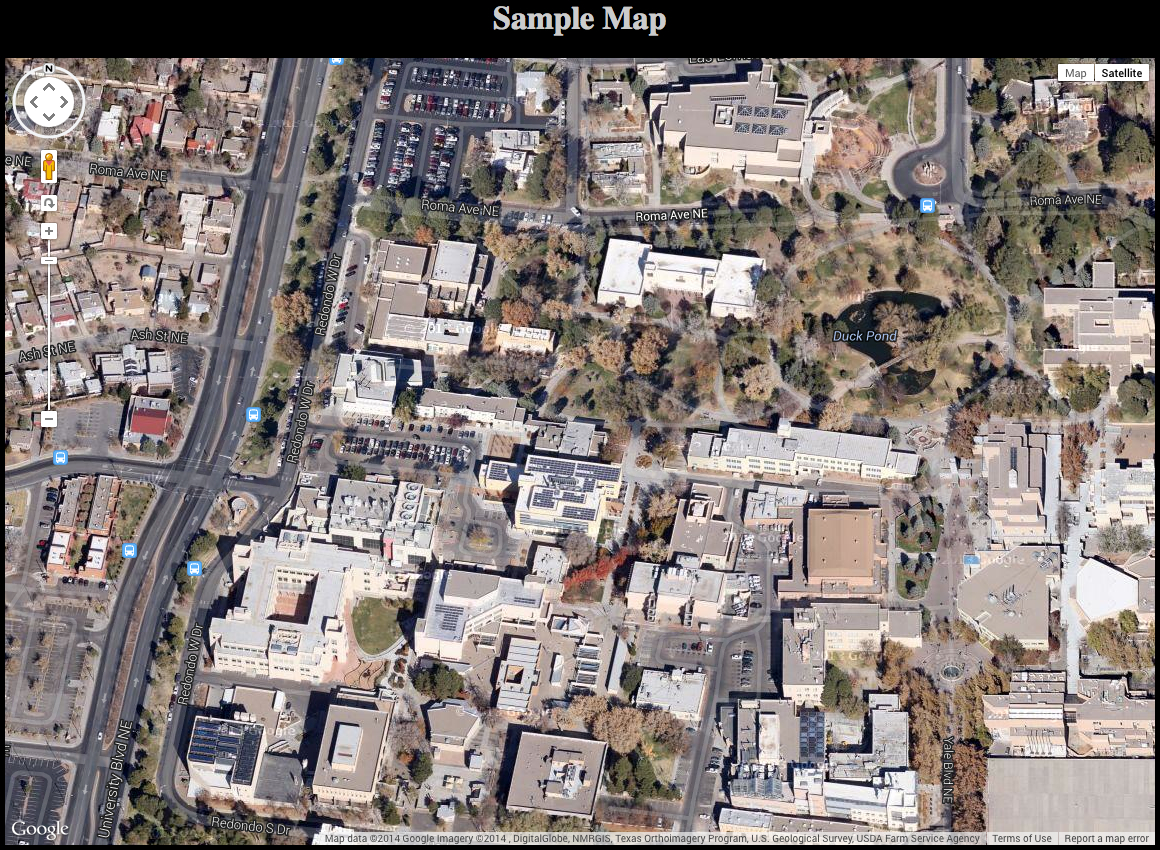
\includegraphics{images/google_05.jpg}~

\url{http://karlbenedict.com/presentations/2014-04-NMGIC/examples/gmaps05.html}

\hyperdef{}{hybridZoomed}{\label{hybridZoomed}}
\begin{Shaded}
\begin{Highlighting}[numbers=left,,]
\DataTypeTok{<!DOCTYPE }\NormalTok{html}\DataTypeTok{>}
\KeywordTok{<html>}
    \KeywordTok{<head>}
        \KeywordTok{<style}\OtherTok{ type=}\StringTok{"text/css"}\KeywordTok{>}
          \NormalTok{html }\KeywordTok{\{} \KeywordTok{height:} \DataTypeTok{100%} \KeywordTok{\}}
          \NormalTok{body }\KeywordTok{\{} \KeywordTok{height:} \DataTypeTok{100%}\KeywordTok{;} 
            \KeywordTok{margin:} \DataTypeTok{0px}\KeywordTok{;} 
            \KeywordTok{padding:} \DataTypeTok{0px}\KeywordTok{;} 
            \KeywordTok{background-color:} \DataTypeTok{black}\KeywordTok{;} 
            \KeywordTok{color:} \DataTypeTok{#CCCCCC}\KeywordTok{;}
            \KeywordTok{text-align:} \DataTypeTok{center}\KeywordTok{\}}
          \FloatTok{#map_canvas} \KeywordTok{\{} \KeywordTok{width:}\DataTypeTok{90%}\KeywordTok{;} 
            \KeywordTok{height:}\DataTypeTok{80%}\KeywordTok{;} 
            \KeywordTok{margin-left:} \DataTypeTok{auto}\KeywordTok{;} 
            \KeywordTok{margin-right:} \DataTypeTok{auto} \KeywordTok{\}}
        \KeywordTok{</style>}
        \KeywordTok{<script}\OtherTok{ type=}\StringTok{"text/javascript"}
\OtherTok{            src=}\StringTok{"http://maps.google.com/maps/api/js?sensor=false"}\KeywordTok{>}
        \KeywordTok{</script>}
        \KeywordTok{<script}\OtherTok{ type=}\StringTok{"text/javascript"}\KeywordTok{>}
\ErrorTok{          function initialize() \{}
\ErrorTok{            var classroom = new google.maps.LatLng(35.084280,-106.624073)}
            \KeywordTok{var} \NormalTok{myOptions = \{}
              \DataTypeTok{zoom}\NormalTok{: }\DecValTok{18}\NormalTok{,}
              \DataTypeTok{center}\NormalTok{: classroom,}
              \DataTypeTok{mapTypeId}\NormalTok{: }\OtherTok{google}\NormalTok{.}\OtherTok{maps}\NormalTok{.}\OtherTok{MapTypeId}\NormalTok{.}\FunctionTok{HYBRID}
            \NormalTok{\};}
\ErrorTok{            var map = new google.maps.Map(}
\ErrorTok{                document.getElementById("map_canvas"),}
                \NormalTok{myOptions);}
          \NormalTok{\}}
        \KeywordTok{</script>}
    \KeywordTok{</head>}
    
    \KeywordTok{<body}\OtherTok{ onload=}\StringTok{"initialize()"}\KeywordTok{>}
      \KeywordTok{<h1>}\NormalTok{Sample Map}\KeywordTok{</h1>}
      \KeywordTok{<div}\OtherTok{ id=}\StringTok{"map_canvas"}\KeywordTok{></div>}
    \KeywordTok{</body>}

\KeywordTok{</html>}
\end{Highlighting}
\end{Shaded}

\subsubsection{Simple - Zoomed - Modified
Controls}\label{simple---zoomed---modified-controls}

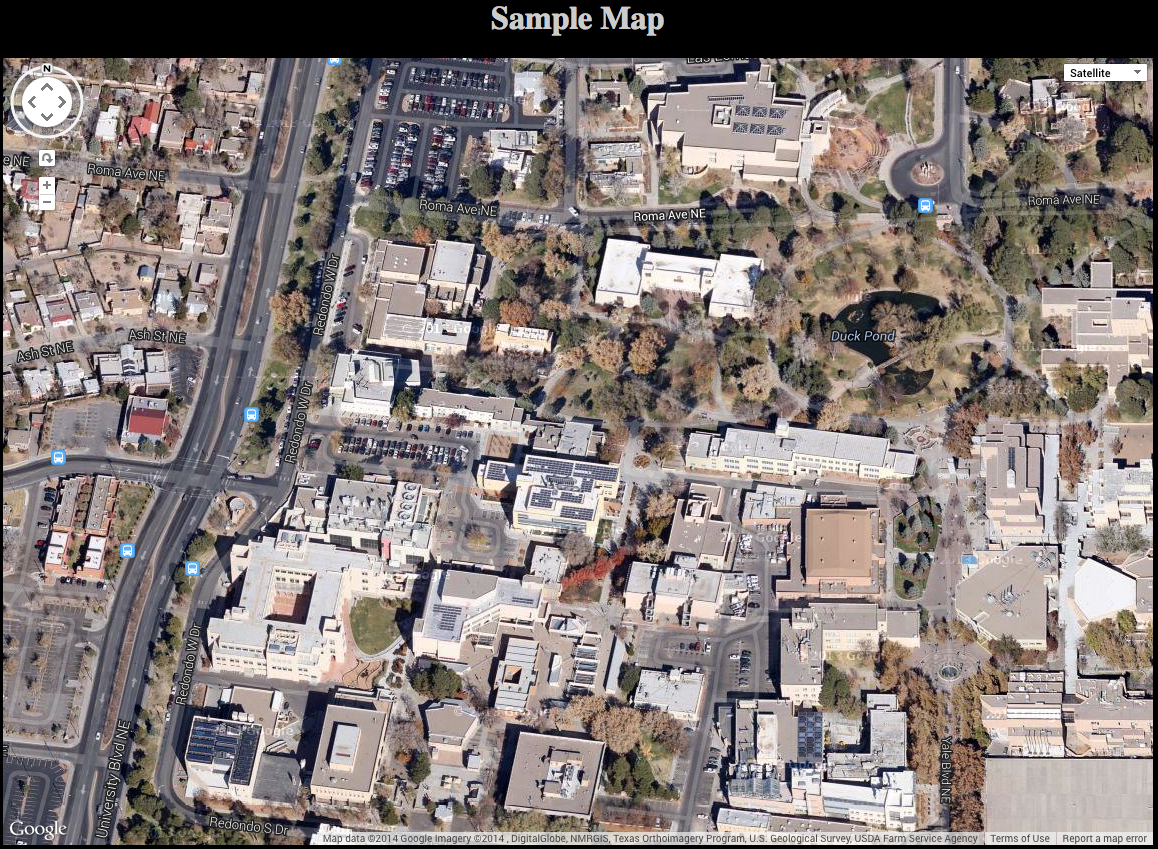
\includegraphics{images/google_06.jpg}~

\url{http://karlbenedict.com/presentations/2014-04-NMGIC/examples/gmaps06.html}

\hyperdef{}{hybridZoomedControls}{\label{hybridZoomedControls}}
\begin{Shaded}
\begin{Highlighting}[numbers=left,,]
\DataTypeTok{<!DOCTYPE }\NormalTok{html}\DataTypeTok{>}
\KeywordTok{<html>}
    \KeywordTok{<head>}
        \KeywordTok{<style}\OtherTok{ type=}\StringTok{"text/css"}\KeywordTok{>}
          \NormalTok{html }\KeywordTok{\{} \KeywordTok{height:} \DataTypeTok{100%} \KeywordTok{\}}
          \NormalTok{body }\KeywordTok{\{} \KeywordTok{height:} \DataTypeTok{100%}\KeywordTok{;} 
            \KeywordTok{margin:} \DataTypeTok{0px}\KeywordTok{;} 
            \KeywordTok{padding:} \DataTypeTok{0px}\KeywordTok{;} 
            \KeywordTok{background-color:} \DataTypeTok{black}\KeywordTok{;} 
            \KeywordTok{color:} \DataTypeTok{#CCCCCC}\KeywordTok{;}
            \KeywordTok{text-align:} \DataTypeTok{center}\KeywordTok{\}}
          \FloatTok{#map_canvas} \KeywordTok{\{} \KeywordTok{width:}\DataTypeTok{90%}\KeywordTok{;} 
            \KeywordTok{height:}\DataTypeTok{80%}\KeywordTok{;} 
            \KeywordTok{margin-left:} \DataTypeTok{auto}\KeywordTok{;} 
            \KeywordTok{margin-right:} \DataTypeTok{auto} \KeywordTok{\}}
        \KeywordTok{</style>}
        \KeywordTok{<script}\OtherTok{ type=}\StringTok{"text/javascript"}
\OtherTok{            src=}\StringTok{"http://maps.google.com/maps/api/js?sensor=false"}\KeywordTok{>}
        \KeywordTok{</script>}
        \KeywordTok{<script}\OtherTok{ type=}\StringTok{"text/javascript"}\KeywordTok{>}
\ErrorTok{          function initialize() \{}
\ErrorTok{            var classroom = new google.maps.LatLng(35.084280,-106.624073)}
            \KeywordTok{var} \NormalTok{myOptions = \{}
              \DataTypeTok{zoom}\NormalTok{: }\DecValTok{18}\NormalTok{,}
              \DataTypeTok{center}\NormalTok{: classroom,}
              \DataTypeTok{mapTypeId}\NormalTok{: }\OtherTok{google}\NormalTok{.}\OtherTok{maps}\NormalTok{.}\OtherTok{MapTypeId}\NormalTok{.}\FunctionTok{HYBRID}\NormalTok{,}
              \DataTypeTok{zoomControl}\NormalTok{: }\KeywordTok{true}\NormalTok{,}
              \DataTypeTok{zoomControlOptions}\NormalTok{: \{}\DataTypeTok{style}\NormalTok{: }\OtherTok{google}\NormalTok{.}\OtherTok{maps}\NormalTok{.}\OtherTok{ZoomControlStyle}\NormalTok{.}\FunctionTok{SMALL}\NormalTok{\},}
              \DataTypeTok{mapTypeControl}\NormalTok{: }\KeywordTok{true}\NormalTok{,}
              \DataTypeTok{mapTypeControlOptions}\NormalTok{: \{}
                \DataTypeTok{style}\NormalTok{: }\OtherTok{google}\NormalTok{.}\OtherTok{maps}\NormalTok{.}\OtherTok{MapTypeControlStyle}\NormalTok{.}\FunctionTok{DROPDOWN_MENU}\NormalTok{\},}
              \DataTypeTok{streetViewControl}\NormalTok{: }\KeywordTok{false}
            \NormalTok{\};}
\ErrorTok{            var map = new google.maps.Map(}
\ErrorTok{                document.getElementById("map_canvas"),}
                \NormalTok{myOptions);}
          \NormalTok{\}}
        \KeywordTok{</script>}
    \KeywordTok{</head>}

    \KeywordTok{<body}\OtherTok{ onload=}\StringTok{"initialize()"}\KeywordTok{>}
      \KeywordTok{<h1>}\NormalTok{Sample Map}\KeywordTok{</h1>}
      \KeywordTok{<div}\OtherTok{ id=}\StringTok{"map_canvas"}\KeywordTok{></div>}
    \KeywordTok{</body>}

\KeywordTok{</html>}
\end{Highlighting}
\end{Shaded}

\subsubsection{Markers}\label{markers}

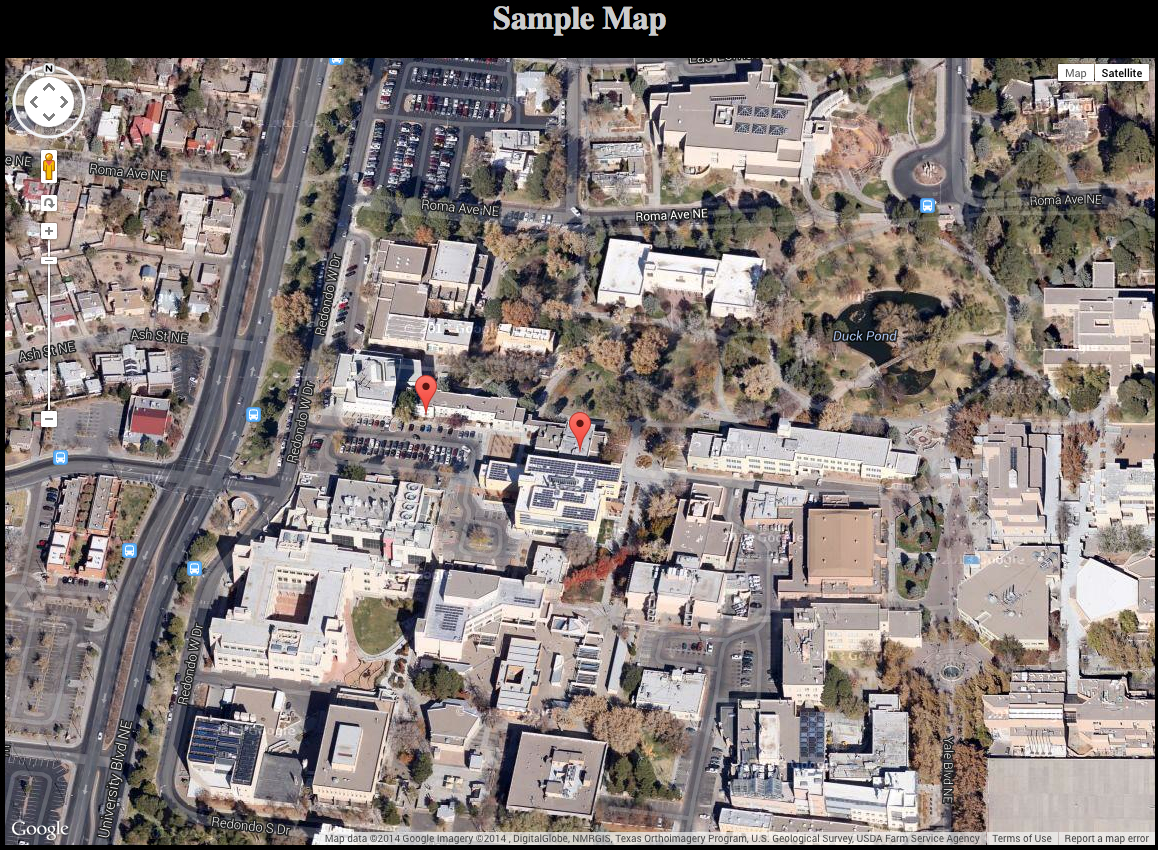
\includegraphics{images/google_07.jpg}~

\url{http://karlbenedict.com/presentations/2014-04-NMGIC/examples/gmaps07.html}

\hyperdef{}{markers}{\label{markers}}
\begin{Shaded}
\begin{Highlighting}[numbers=left,,]
\DataTypeTok{<!DOCTYPE }\NormalTok{html}\DataTypeTok{>}
\KeywordTok{<html>}
    \KeywordTok{<head>}
        \KeywordTok{<style}\OtherTok{ type=}\StringTok{"text/css"}\KeywordTok{>}
          \NormalTok{html }\KeywordTok{\{} \KeywordTok{height:} \DataTypeTok{100%} \KeywordTok{\}}
          \NormalTok{body }\KeywordTok{\{} \KeywordTok{height:} \DataTypeTok{100%}\KeywordTok{;} 
            \KeywordTok{margin:} \DataTypeTok{0px}\KeywordTok{;} 
            \KeywordTok{padding:} \DataTypeTok{0px}\KeywordTok{;} 
            \KeywordTok{background-color:} \DataTypeTok{black}\KeywordTok{;} 
            \KeywordTok{color:} \DataTypeTok{#CCCCCC}\KeywordTok{;}
            \KeywordTok{text-align:} \DataTypeTok{center}\KeywordTok{\}}
          \FloatTok{#map_canvas} \KeywordTok{\{} \KeywordTok{width:}\DataTypeTok{90%}\KeywordTok{;} 
            \KeywordTok{height:}\DataTypeTok{80%}\KeywordTok{;} 
            \KeywordTok{margin-left:} \DataTypeTok{auto}\KeywordTok{;} 
            \KeywordTok{margin-right:} \DataTypeTok{auto} \KeywordTok{\}}
        \KeywordTok{</style>}
        \KeywordTok{<script}\OtherTok{ type=}\StringTok{"text/javascript"}
\OtherTok{            src=}\StringTok{"http://maps.google.com/maps/api/js?sensor=false"}\KeywordTok{>}
        \KeywordTok{</script>}
        \KeywordTok{<script}\OtherTok{ type=}\StringTok{"text/javascript"}\KeywordTok{>}
\ErrorTok{          function initialize() \{}
\ErrorTok{            var classroom = new google.maps.LatLng(35.084280,-106.624073)}
\ErrorTok{            var office = new google.maps.LatLng(35.084506,-106.624899)}
            \KeywordTok{var} \NormalTok{myOptions = \{}
              \DataTypeTok{zoom}\NormalTok{: }\DecValTok{18}\NormalTok{,}
              \DataTypeTok{center}\NormalTok{: classroom,}
              \DataTypeTok{mapTypeId}\NormalTok{: }\OtherTok{google}\NormalTok{.}\OtherTok{maps}\NormalTok{.}\OtherTok{MapTypeId}\NormalTok{.}\FunctionTok{HYBRID}
              \NormalTok{\};}
\ErrorTok{            var map = new google.maps.Map(}
\ErrorTok{              document.getElementById("map_canvas"), }
              \NormalTok{myOptions);}
            
\ErrorTok{            var classroomMarker = new google.maps.Marker(\{}
              \NormalTok{position: classroom,}
              \NormalTok{title:}\StringTok{"Geography 485L/585L Classroom, Bandelier East, Room 106"}
              \NormalTok{\});}
\ErrorTok{            classroomMarker.setMap(map);}
            
\ErrorTok{            var officeMarker = new google.maps.Marker(\{}
              \NormalTok{position: office,}
              \NormalTok{title:}\StringTok{"Office, Bandelier West, Room 107"}
              \NormalTok{\});}
\ErrorTok{            officeMarker.setMap(map); }
          \NormalTok{\}}
        \KeywordTok{</script>}
    \KeywordTok{</head>}
    
    \KeywordTok{<body}\OtherTok{ onload=}\StringTok{"initialize()"}\KeywordTok{>}
      \KeywordTok{<h1>}\NormalTok{Sample Map}\KeywordTok{</h1>}
      \KeywordTok{<div}\OtherTok{ id=}\StringTok{"map_canvas"}\KeywordTok{></div>}
    \KeywordTok{</body>}

\KeywordTok{</html>}
\end{Highlighting}
\end{Shaded}

\subsubsection{Polyline}\label{polyline}

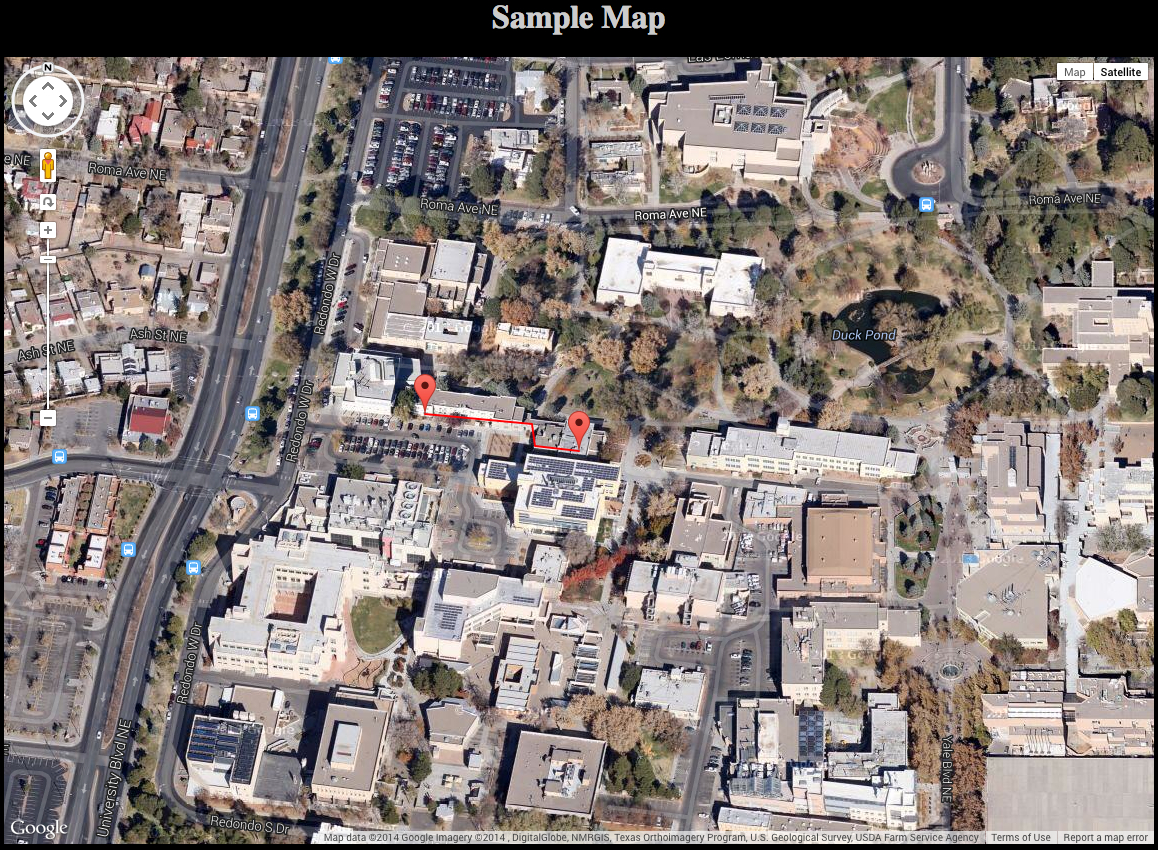
\includegraphics{images/google_08.jpg}~

\url{http://karlbenedict.com/presentations/2014-04-NMGIC/examples/gmaps08.html}

\hyperdef{}{polyline}{\label{polyline}}
\begin{Shaded}
\begin{Highlighting}[numbers=left,,]
\DataTypeTok{<!DOCTYPE }\NormalTok{html}\DataTypeTok{>}
\KeywordTok{<html>}
    \KeywordTok{<head>}
        \KeywordTok{<style}\OtherTok{ type=}\StringTok{"text/css"}\KeywordTok{>}
          \NormalTok{html }\KeywordTok{\{} \KeywordTok{height:} \DataTypeTok{100%} \KeywordTok{\}}
          \NormalTok{body }\KeywordTok{\{} \KeywordTok{height:} \DataTypeTok{100%}\KeywordTok{;} 
            \KeywordTok{margin:} \DataTypeTok{0px}\KeywordTok{;} 
            \KeywordTok{padding:} \DataTypeTok{0px}\KeywordTok{;} 
            \KeywordTok{background-color:} \DataTypeTok{black}\KeywordTok{;} 
            \KeywordTok{color:} \DataTypeTok{#CCCCCC}\KeywordTok{;}
            \KeywordTok{text-align:} \DataTypeTok{center}\KeywordTok{\}}
          \FloatTok{#map_canvas} \KeywordTok{\{} \KeywordTok{width:}\DataTypeTok{90%}\KeywordTok{;} 
            \KeywordTok{height:}\DataTypeTok{80%}\KeywordTok{;} 
            \KeywordTok{margin-left:} 
            \DataTypeTok{auto}\KeywordTok{;} 
            \KeywordTok{margin-right:} \DataTypeTok{auto} \KeywordTok{\}}
        \KeywordTok{</style>}
        \KeywordTok{<script}\OtherTok{ type=}\StringTok{"text/javascript"}
\OtherTok{            src=}\StringTok{"http://maps.google.com/maps/api/js?sensor=false"}\KeywordTok{>}
        \KeywordTok{</script>}
        \KeywordTok{<script}\OtherTok{ type=}\StringTok{"text/javascript"}\KeywordTok{>}
\ErrorTok{          function initialize() \{}
\ErrorTok{            var classroom = new google.maps.LatLng(35.084280,-106.624073)}
\ErrorTok{            var office = new google.maps.LatLng(35.084506,-106.624899)}
            \KeywordTok{var} \NormalTok{myOptions = \{}
              \DataTypeTok{zoom}\NormalTok{: }\DecValTok{18}\NormalTok{,}
              \DataTypeTok{center}\NormalTok{: classroom,}
              \DataTypeTok{mapTypeId}\NormalTok{: }\OtherTok{google}\NormalTok{.}\OtherTok{maps}\NormalTok{.}\OtherTok{MapTypeId}\NormalTok{.}\FunctionTok{HYBRID}
              \NormalTok{\};}
\ErrorTok{            var map = new google.maps.Map(}
\ErrorTok{              document.getElementById("map_canvas"), }
              \NormalTok{myOptions);}
        
\ErrorTok{            var classroomMarker = new google.maps.Marker(\{}
              \NormalTok{position: classroom,}
              \NormalTok{title:}\StringTok{"Geography 485L/585L Classroom, Bandelier East, Room 106"}
              \NormalTok{\});}
\ErrorTok{            classroomMarker.setMap(map);}
        
\ErrorTok{            var officeMarker = new google.maps.Marker(\{}
              \NormalTok{position: office,}
              \NormalTok{title:}\StringTok{"Office, Bandelier West, Room 107"}
              \NormalTok{\});}
\ErrorTok{            officeMarker.setMap(map); }
        
            \KeywordTok{var} \NormalTok{officeVisitCoordinates = [}
              \NormalTok{office,}
\ErrorTok{              new google.maps.LatLng(35.084445,-106.624327),}
\ErrorTok{              new google.maps.LatLng(35.084309,-106.624308),}
              \NormalTok{classroom}
              \NormalTok{];}
\ErrorTok{            var officePath = new google.maps.Polyline(\{}
              \NormalTok{path: officeVisitCoordinates,}
              \NormalTok{strokeColor: }\StringTok{"#FF0000"}\NormalTok{,}
              \NormalTok{strokeOpacity: }\FloatTok{1.0}\NormalTok{,}
              \NormalTok{strokeWeight: }\DecValTok{2}
\ErrorTok{            \});}
\ErrorTok{            officePath.setMap(map)}
\ErrorTok{          \}}
        \NormalTok{<}\OtherTok{/script>}
\OtherTok{    </head}\NormalTok{>}

    \NormalTok{<body onload=}\StringTok{"initialize()"}\NormalTok{>}
      \NormalTok{<h1>Sample Map<}\OtherTok{/h1>}
\OtherTok{      <div id="map_canvas"></div}\NormalTok{>}
    \NormalTok{<}\OtherTok{/body>}

\OtherTok{</html}\NormalTok{>}
\end{Highlighting}
\end{Shaded}

\subsubsection{Polygon}\label{polygon}

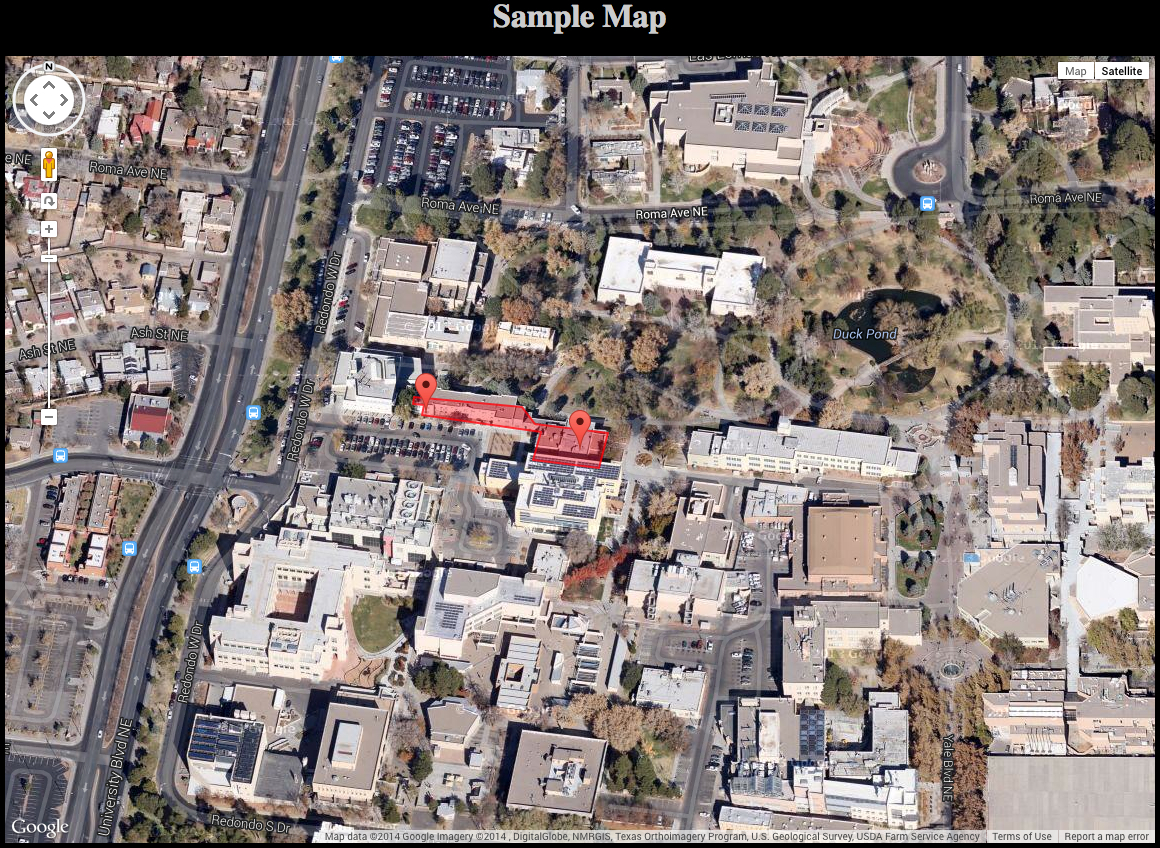
\includegraphics{images/google_09.jpg}~

\url{http://karlbenedict.com/presentations/2014-04-NMGIC/examples/gmaps09.html}

\hyperdef{}{polygon}{\label{polygon}}
\begin{Shaded}
\begin{Highlighting}[numbers=left,,]
\DataTypeTok{<!DOCTYPE }\NormalTok{html}\DataTypeTok{>}
\KeywordTok{<html>}
    \KeywordTok{<head>}
        \KeywordTok{<style}\OtherTok{ type=}\StringTok{"text/css"}\KeywordTok{>}
          \NormalTok{html }\KeywordTok{\{} \KeywordTok{height:} \DataTypeTok{100%} \KeywordTok{\}}
          \NormalTok{body }\KeywordTok{\{} \KeywordTok{height:} \DataTypeTok{100%}\KeywordTok{;} 
            \KeywordTok{margin:} \DataTypeTok{0px}\KeywordTok{;} 
            \KeywordTok{padding:} \DataTypeTok{0px}\KeywordTok{;} 
            \KeywordTok{background-color:} \DataTypeTok{black}\KeywordTok{;} 
            \KeywordTok{color:} \DataTypeTok{#CCCCCC}\KeywordTok{;}
            \KeywordTok{text-align:} \DataTypeTok{center}\KeywordTok{\}}
          \FloatTok{#map_canvas} \KeywordTok{\{} \KeywordTok{width:}\DataTypeTok{90%}\KeywordTok{;} 
            \KeywordTok{height:}\DataTypeTok{80%}\KeywordTok{;} 
            \KeywordTok{margin-left:} \DataTypeTok{auto}\KeywordTok{;} 
            \KeywordTok{margin-right:} \DataTypeTok{auto} \KeywordTok{\}}
        \KeywordTok{</style>}
        \KeywordTok{<script}\OtherTok{ type=}\StringTok{"text/javascript"}
\OtherTok{            src=}\StringTok{"http://maps.google.com/maps/api/js?sensor=false"}\KeywordTok{>}
        \KeywordTok{</script>}
        \KeywordTok{<script}\OtherTok{ type=}\StringTok{"text/javascript"}\KeywordTok{>}
\ErrorTok{          function initialize() \{}
\ErrorTok{            var classroom = new google.maps.LatLng(35.084280,-106.624073)}
\ErrorTok{            var office = new google.maps.LatLng(35.084506,-106.624899)}
            \KeywordTok{var} \NormalTok{myOptions = \{}
              \DataTypeTok{zoom}\NormalTok{: }\DecValTok{18}\NormalTok{,}
              \DataTypeTok{center}\NormalTok{: classroom,}
              \DataTypeTok{mapTypeId}\NormalTok{: }\OtherTok{google}\NormalTok{.}\OtherTok{maps}\NormalTok{.}\OtherTok{MapTypeId}\NormalTok{.}\FunctionTok{HYBRID}
              \NormalTok{\};}
\ErrorTok{            var map = new google.maps.Map(}
\ErrorTok{              document.getElementById("map_canvas"), }
              \NormalTok{myOptions);}
\ErrorTok{            var classroomMarker = new google.maps.Marker(\{}
              \NormalTok{position: classroom,}
              \NormalTok{title:}\StringTok{"Geography 485L/585L Classroom, Bandelier East, Room 106"}
              \NormalTok{\});}
\ErrorTok{            classroomMarker.setMap(map);}
\ErrorTok{            var officeMarker = new google.maps.Marker(\{}
              \NormalTok{position: office,}
              \NormalTok{title:}\StringTok{"Office, Bandelier West, Room 107"}
              \NormalTok{\});}
\ErrorTok{            officeMarker.setMap(map); }
            \KeywordTok{var} \NormalTok{buildingCoordinates = [}
\ErrorTok{              new google.maps.LatLng(35.084498,-106.624921),}
\ErrorTok{              new google.maps.LatLng(35.084558,-106.624911),}
\ErrorTok{              new google.maps.LatLng(35.084566,-106.624970),}
\ErrorTok{              new google.maps.LatLng(35.084609,-106.624966),}
\ErrorTok{              new google.maps.LatLng(35.084544,-106.624383),}
\ErrorTok{              new google.maps.LatLng(35.084438,-106.624317),}
\ErrorTok{              new google.maps.LatLng(35.084384,-106.623922),}
\ErrorTok{              new google.maps.LatLng(35.084164,-106.623970),}
\ErrorTok{              new google.maps.LatLng(35.084214,-106.624324),}
\ErrorTok{              new google.maps.LatLng(35.084214,-106.624324),}
\ErrorTok{              new google.maps.LatLng(35.084391,-106.624284)}
              \NormalTok{];}
\ErrorTok{            var bldgPoly = new google.maps.Polygon(\{}
              \NormalTok{paths: buildingCoordinates,}
              \NormalTok{strokeColor: }\StringTok{"#FF0000"}\NormalTok{,}
              \NormalTok{strokeOpacity: }\FloatTok{0.8}\NormalTok{,}
              \NormalTok{strokeWeight: }\DecValTok{2}\NormalTok{,}
              \NormalTok{fillColor: }\StringTok{"#FF0000"}\NormalTok{,}
              \NormalTok{fillOpacity: }\FloatTok{0.35}
\ErrorTok{            \});}
\ErrorTok{            bldgPoly.setMap(map)}
\ErrorTok{          \}}
        \NormalTok{<}\OtherTok{/script>}
\OtherTok{    </head}\NormalTok{>}
    
    \NormalTok{<body onload=}\StringTok{"initialize()"}\NormalTok{>}
      \NormalTok{<h1>Sample Map<}\OtherTok{/h1>}
\OtherTok{      <div id="map_canvas"></div}\NormalTok{>}
    \NormalTok{<}\OtherTok{/body>}

\OtherTok{</html}\NormalTok{>}
\end{Highlighting}
\end{Shaded}

\subsubsection{Adding an Info Window}\label{adding-an-info-window}

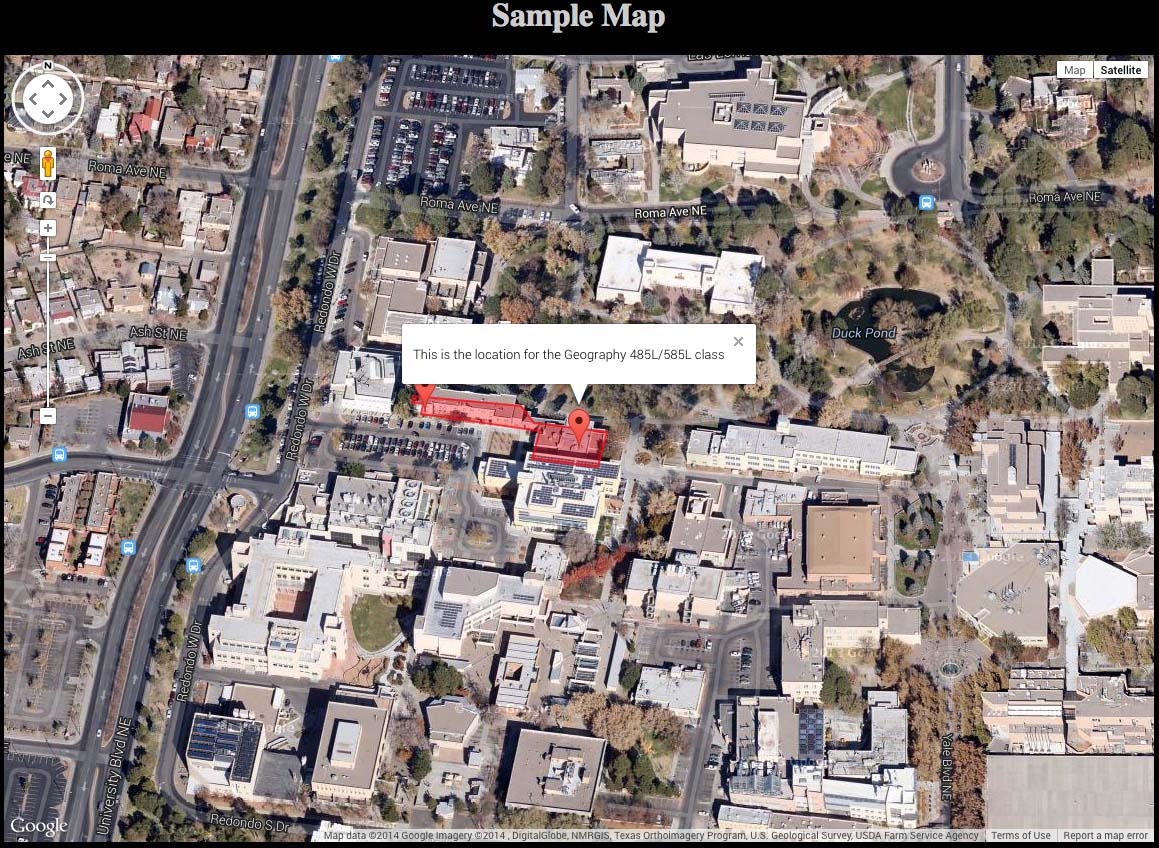
\includegraphics{images/google_10.jpg}~

\url{http://karlbenedict.com/presentations/2014-04-NMGIC/examples/gmaps10.html}

\hyperdef{}{infoWindow}{\label{infoWindow}}
\begin{Shaded}
\begin{Highlighting}[numbers=left,,]
\DataTypeTok{<!DOCTYPE }\NormalTok{html}\DataTypeTok{>}
\KeywordTok{<html>}
    \KeywordTok{<head>}
        \KeywordTok{<style}\OtherTok{ type=}\StringTok{"text/css"}\KeywordTok{>}
          \NormalTok{html }\KeywordTok{\{} \KeywordTok{height:} \DataTypeTok{100%} \KeywordTok{\}}
          \NormalTok{body }\KeywordTok{\{} \KeywordTok{height:} \DataTypeTok{100%}\KeywordTok{;} 
            \KeywordTok{margin:} \DataTypeTok{0px}\KeywordTok{;} 
            \KeywordTok{padding:} \DataTypeTok{0px}\KeywordTok{;} 
            \KeywordTok{background-color:} \DataTypeTok{black}\KeywordTok{;} 
            \KeywordTok{color:} \DataTypeTok{#CCCCCC}\KeywordTok{;}
            \KeywordTok{text-align:} \DataTypeTok{center}\KeywordTok{\}}
          \FloatTok{#map_canvas} \KeywordTok{\{} \KeywordTok{width:}\DataTypeTok{90%}\KeywordTok{;} 
            \KeywordTok{height:}\DataTypeTok{80%}\KeywordTok{;} 
            \KeywordTok{margin-left:} \DataTypeTok{auto}\KeywordTok{;} 
            \KeywordTok{margin-right:} \DataTypeTok{auto} \KeywordTok{\}}
          \FloatTok{.infoBox} \KeywordTok{\{} \KeywordTok{color:}\DataTypeTok{black} \KeywordTok{\}}
        \KeywordTok{</style>}
        \KeywordTok{<script}\OtherTok{ type=}\StringTok{"text/javascript"}
\OtherTok{            src=}\StringTok{"http://maps.google.com/maps/api/js?sensor=false"}\KeywordTok{>}
        \KeywordTok{</script>}
        \KeywordTok{<script}\OtherTok{ type=}\StringTok{"text/javascript"}\KeywordTok{>}
\ErrorTok{          function initialize() \{}
\ErrorTok{            var classroom = new google.maps.LatLng(35.084280,-106.624073)}
\ErrorTok{            var office = new google.maps.LatLng(35.084506,-106.624899)}
            \KeywordTok{var} \NormalTok{myOptions = \{}
              \DataTypeTok{zoom}\NormalTok{: }\DecValTok{18}\NormalTok{,}
              \DataTypeTok{center}\NormalTok{: classroom,}
              \DataTypeTok{mapTypeId}\NormalTok{: }\OtherTok{google}\NormalTok{.}\OtherTok{maps}\NormalTok{.}\OtherTok{MapTypeId}\NormalTok{.}\FunctionTok{HYBRID}
              \NormalTok{\};}
\ErrorTok{            var map = new google.maps.Map(}
\ErrorTok{              document.getElementById("map_canvas"), }
              \NormalTok{myOptions);}
\ErrorTok{            var classroomMarker = new google.maps.Marker(\{}
              \NormalTok{position: classroom,}
              \NormalTok{title:}\StringTok{"Geography 485L/585L Classroom, Bandelier East, Room 106"}
              \NormalTok{\});}
\ErrorTok{            classroomMarker.setMap(map);}
\ErrorTok{            var officeMarker = new google.maps.Marker(\{}
              \NormalTok{position: office,}
              \NormalTok{title:}\StringTok{"Office, Bandelier West, Room 107"}
              \NormalTok{\});}
\ErrorTok{            officeMarker.setMap(map); }
            \KeywordTok{var} \NormalTok{buildingCoordinates = [}
\ErrorTok{              new google.maps.LatLng(35.084498,-106.624921),}
\ErrorTok{              new google.maps.LatLng(35.084558,-106.624911),}
\ErrorTok{              new google.maps.LatLng(35.084566,-106.624970),}
\ErrorTok{              new google.maps.LatLng(35.084609,-106.624966),}
\ErrorTok{              new google.maps.LatLng(35.084544,-106.624383),}
\ErrorTok{              new google.maps.LatLng(35.084438,-106.624317),}
\ErrorTok{              new google.maps.LatLng(35.084384,-106.623922),}
\ErrorTok{              new google.maps.LatLng(35.084164,-106.623970),}
\ErrorTok{              new google.maps.LatLng(35.084214,-106.624324),}
\ErrorTok{              new google.maps.LatLng(35.084214,-106.624324),}
\ErrorTok{              new google.maps.LatLng(35.084391,-106.624284)}
              \NormalTok{];}
\ErrorTok{            var bldgPoly = new google.maps.Polygon(\{}
              \NormalTok{paths: buildingCoordinates,}
              \NormalTok{strokeColor: }\StringTok{"#FF0000"}\NormalTok{,}
              \NormalTok{strokeOpacity: }\FloatTok{0.8}\NormalTok{,}
              \NormalTok{strokeWeight: }\DecValTok{2}\NormalTok{,}
              \NormalTok{fillColor: }\StringTok{"#FF0000"}\NormalTok{,}
              \NormalTok{fillOpacity: }\FloatTok{0.35}
\ErrorTok{            \});}
\ErrorTok{            bldgPoly.setMap(map);}
            \KeywordTok{var} \NormalTok{classInfoContent = }\StringTok{'<div class="infoBox">'} \NormalTok{+}
              \StringTok{'<p>This is the location for the Geography 485L/585L class</p>'} \NormalTok{+}
              \StringTok{'</div>'}
\ErrorTok{            var classInfoWindow = new google.maps.InfoWindow(\{}
              \NormalTok{content: classInfoContent}
\ErrorTok{              \});}
\ErrorTok{            google.maps.event.addListener(classroomMarker, 'click', function() \{}
\ErrorTok{              classInfoWindow.open(map,classroomMarker);}
\ErrorTok{              \});}
\ErrorTok{          \}}
        \NormalTok{<}\OtherTok{/script>}
\OtherTok{    </head}\NormalTok{>}
    
    \NormalTok{<body onload=}\StringTok{"initialize()"}\NormalTok{>}
      \NormalTok{<h1>Sample Map<}\OtherTok{/h1>}
\OtherTok{      <div id="map_canvas"></div}\NormalTok{>}
    \NormalTok{<}\OtherTok{/body>}

\OtherTok{</html}\NormalTok{>}
\end{Highlighting}
\end{Shaded}

\subsubsection{\emph{Getting Started with Styled Maps} -
Video}\label{getting-started-with-styled-maps---video}

\href{https://developers.google.com/maps/documentation/javascript/styling}{Styled
Maps Documentation} \textbar{}
\href{http://gmaps-samples-v3.googlecode.com/svn/trunk/styledmaps/wizard/index.html}{Styled
Maps Wizard} \textbar{} \href{http://youtu.be/0hhiEjf7_NA}{YouTube
Introductory Video}

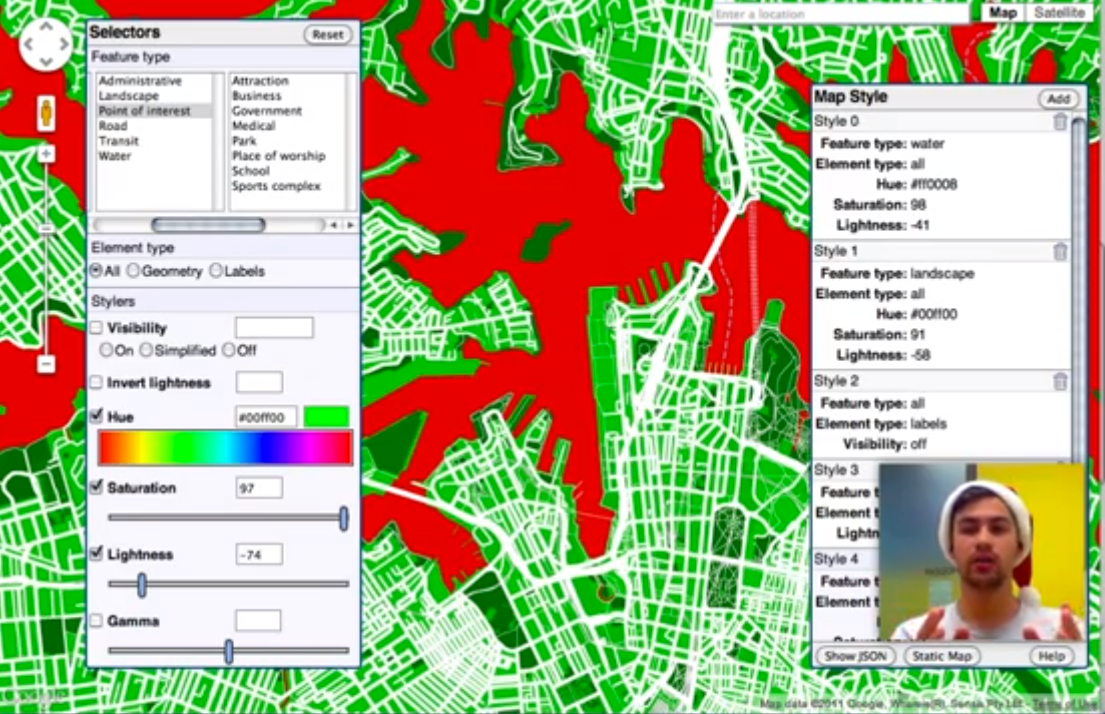
\includegraphics{./images/styledMapsWizard.png}~

\subsubsection{Map Example: Simple -
Styled}\label{map-example-simple---styled}

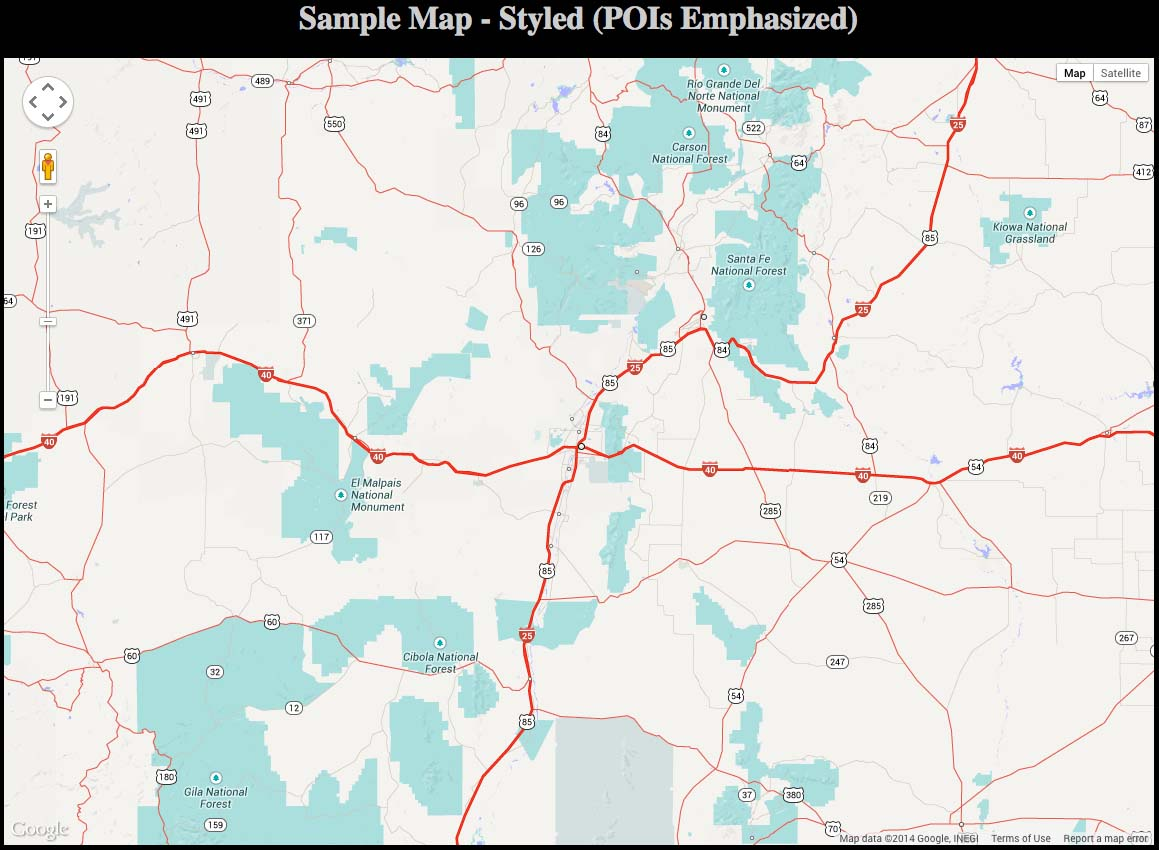
\includegraphics{images/google_11.jpg}~

\url{http://karlbenedict.com/presentations/2014-04-NMGIC/examples/gmaps_styled.html}

\hyperdef{}{styledMap}{\label{styledMap}}
\begin{Shaded}
\begin{Highlighting}[numbers=left,,]
\DataTypeTok{<!DOCTYPE }\NormalTok{html}\DataTypeTok{>}
\KeywordTok{<html>}
\KeywordTok{<head>}
\KeywordTok{<style}\OtherTok{ type=}\StringTok{"text/css"}\KeywordTok{>}
  \NormalTok{html }\KeywordTok{\{} \KeywordTok{height:} \DataTypeTok{100%} \KeywordTok{\}}
  \NormalTok{body }\KeywordTok{\{} \KeywordTok{height:} \DataTypeTok{100%}\KeywordTok{;} 
    \KeywordTok{margin:} \DataTypeTok{0px}\KeywordTok{;} 
    \KeywordTok{padding:} \DataTypeTok{0px}\KeywordTok{;} 
    \KeywordTok{background-color:} \DataTypeTok{black}\KeywordTok{;} 
    \KeywordTok{color:} \DataTypeTok{#CCCCCC}\KeywordTok{;}
    \KeywordTok{text-align:} \DataTypeTok{center}\KeywordTok{\}}
  \FloatTok{#map_canvas} \KeywordTok{\{} \KeywordTok{width:}\DataTypeTok{90%}\KeywordTok{;} 
    \KeywordTok{height:}\DataTypeTok{80%}\KeywordTok{;} 
    \KeywordTok{margin-left:} 
    \DataTypeTok{auto}\KeywordTok{;} 
    \KeywordTok{margin-right:} \DataTypeTok{auto} \KeywordTok{\}}
\KeywordTok{</style>}
\KeywordTok{<script}\OtherTok{ type=}\StringTok{"text/javascript"}
\OtherTok{    src=}\StringTok{"http://maps.google.com/maps/api/js?v=3.2}\ErrorTok{&}\StringTok{sensor=false"}\KeywordTok{>}
\KeywordTok{</script>}
\KeywordTok{<script}\OtherTok{ type=}\StringTok{"text/javascript"}\KeywordTok{>}
\ErrorTok{  function initialize() \{}
\ErrorTok{    var classroom = new google.maps.LatLng(35.084280,-106.624073)}
    \KeywordTok{var} \NormalTok{myOptions = \{}
      \DataTypeTok{zoom}\NormalTok{: }\DecValTok{8}\NormalTok{,}
      \DataTypeTok{center}\NormalTok{: classroom,}
      \DataTypeTok{mapTypeId}\NormalTok{: }\OtherTok{google}\NormalTok{.}\OtherTok{maps}\NormalTok{.}\OtherTok{MapTypeId}\NormalTok{.}\FunctionTok{ROADMAP}\NormalTok{,}
      \DataTypeTok{styles}\NormalTok{: [}
              \NormalTok{\{}
                \DataTypeTok{featureType}\NormalTok{: }\StringTok{"water"}\NormalTok{,}
                \DataTypeTok{stylers}\NormalTok{: [}
                  \NormalTok{\{ }\DataTypeTok{visibility}\NormalTok{: }\StringTok{"on"} \NormalTok{\},}
                  \NormalTok{\{ }\DataTypeTok{hue}\NormalTok{: }\StringTok{"#0008ff"} \NormalTok{\}}
                \NormalTok{]}
              \NormalTok{\},\{}
                \DataTypeTok{featureType}\NormalTok{: }\StringTok{"road.highway"}\NormalTok{,}
                \DataTypeTok{stylers}\NormalTok{: [}
                  \NormalTok{\{ }\DataTypeTok{hue}\NormalTok{: }\StringTok{"#ff1a00"} \NormalTok{\}}
                \NormalTok{]}
              \NormalTok{\},\{}
                \DataTypeTok{featureType}\NormalTok{: }\StringTok{"road.arterial"}\NormalTok{,}
                \DataTypeTok{stylers}\NormalTok{: [}
                  \NormalTok{\{ }\DataTypeTok{hue}\NormalTok{: }\StringTok{"#ffa200"} \NormalTok{\},}
                  \NormalTok{\{ }\DataTypeTok{visibility}\NormalTok{: }\StringTok{"simplified"} \NormalTok{\}}
                \NormalTok{]}
              \NormalTok{\},\{}
                \DataTypeTok{featureType}\NormalTok{: }\StringTok{"road.local"}\NormalTok{,}
                \DataTypeTok{stylers}\NormalTok{: [}
                  \NormalTok{\{ }\DataTypeTok{visibility}\NormalTok{: }\StringTok{"off"} \NormalTok{\}}
                \NormalTok{]}
              \NormalTok{\},\{}
                \DataTypeTok{featureType}\NormalTok{: }\StringTok{"administrative"}\NormalTok{,}
                \DataTypeTok{stylers}\NormalTok{: [}
                  \NormalTok{\{ }\DataTypeTok{visibility}\NormalTok{: }\StringTok{"simplified"} \NormalTok{\}}
                \NormalTok{]}
              \NormalTok{\},\{}
                \DataTypeTok{featureType}\NormalTok{: }\StringTok{"poi"}\NormalTok{,}
                \DataTypeTok{stylers}\NormalTok{: [}
                  \NormalTok{\{ }\DataTypeTok{visibility}\NormalTok{: }\StringTok{"on"} \NormalTok{\},}
                  \NormalTok{\{ }\DataTypeTok{hue}\NormalTok{: }\StringTok{"#00ffff"} \NormalTok{\}}
                \NormalTok{]}
              \NormalTok{\},\{}
                \DataTypeTok{featureType}\NormalTok{: }\StringTok{"poi"}\NormalTok{,}
                \DataTypeTok{stylers}\NormalTok{: [}
                  \NormalTok{\{ }\DataTypeTok{visibility}\NormalTok{: }\StringTok{"on"} \NormalTok{\}}
                \NormalTok{]}
              \NormalTok{\}}
            \NormalTok{]}
    \NormalTok{\};}
\ErrorTok{    var map = new google.maps.Map(document.getElementById("map_canvas"),}
        \NormalTok{myOptions);}
  \NormalTok{\}}
\KeywordTok{</script>}
\KeywordTok{</head>}

\KeywordTok{<body}\OtherTok{ onload=}\StringTok{"initialize()"}\KeywordTok{>}
  \KeywordTok{<h1>}\NormalTok{Sample Map - Styled (POIs Emphasized)}\KeywordTok{</h1>}
  \KeywordTok{<div}\OtherTok{ id=}\StringTok{"map_canvas"}\KeywordTok{></div>}
\KeywordTok{</body>}

\KeywordTok{</html>}
\end{Highlighting}
\end{Shaded}

\subsubsection{\emph{Google I/O 2011: Managing and visualizing your
geospatial data with Fusion Tables} -
Video}\label{google-io-2011-managing-and-visualizing-your-geospatial-data-with-fusion-tables---video}

\href{http://youtu.be/Z2o0mtnF1Bg}{Fusion Tables Introduction Video} -
Some particularly relevant sections:
\href{http://youtu.be/Z2o0mtnF1Bg}{Introduction (0:00 - 10:30)}
\textbar{} \href{http://youtu.be/Z2o0mtnF1Bg?t=21m40s}{Google Maps API
Integration (21:40 - 34:42)} \textbar{}
\href{http://youtu.be/Z2o0mtnF1Bg?t=52m}{Summary and Links (52:00 -
52:40)}

\href{http://tinyurl.com/nxlgcwq}{Fusion Tables Documentation/Help}

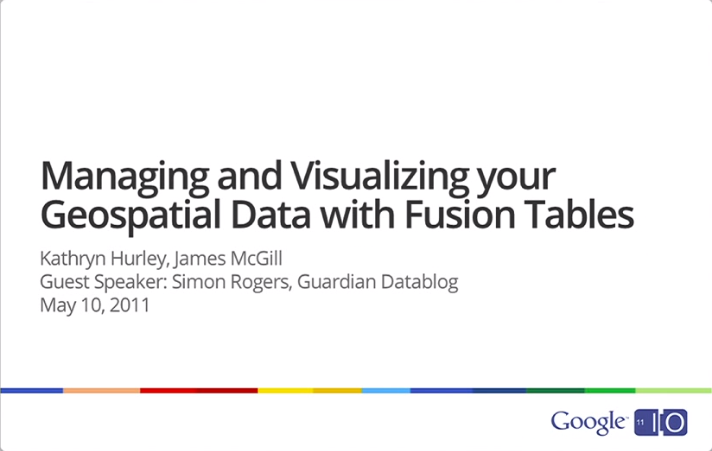
\includegraphics{./images/fusionTablesVideo.png}~

\subsubsection{Bringing It All Together}\label{bringing-it-all-together}

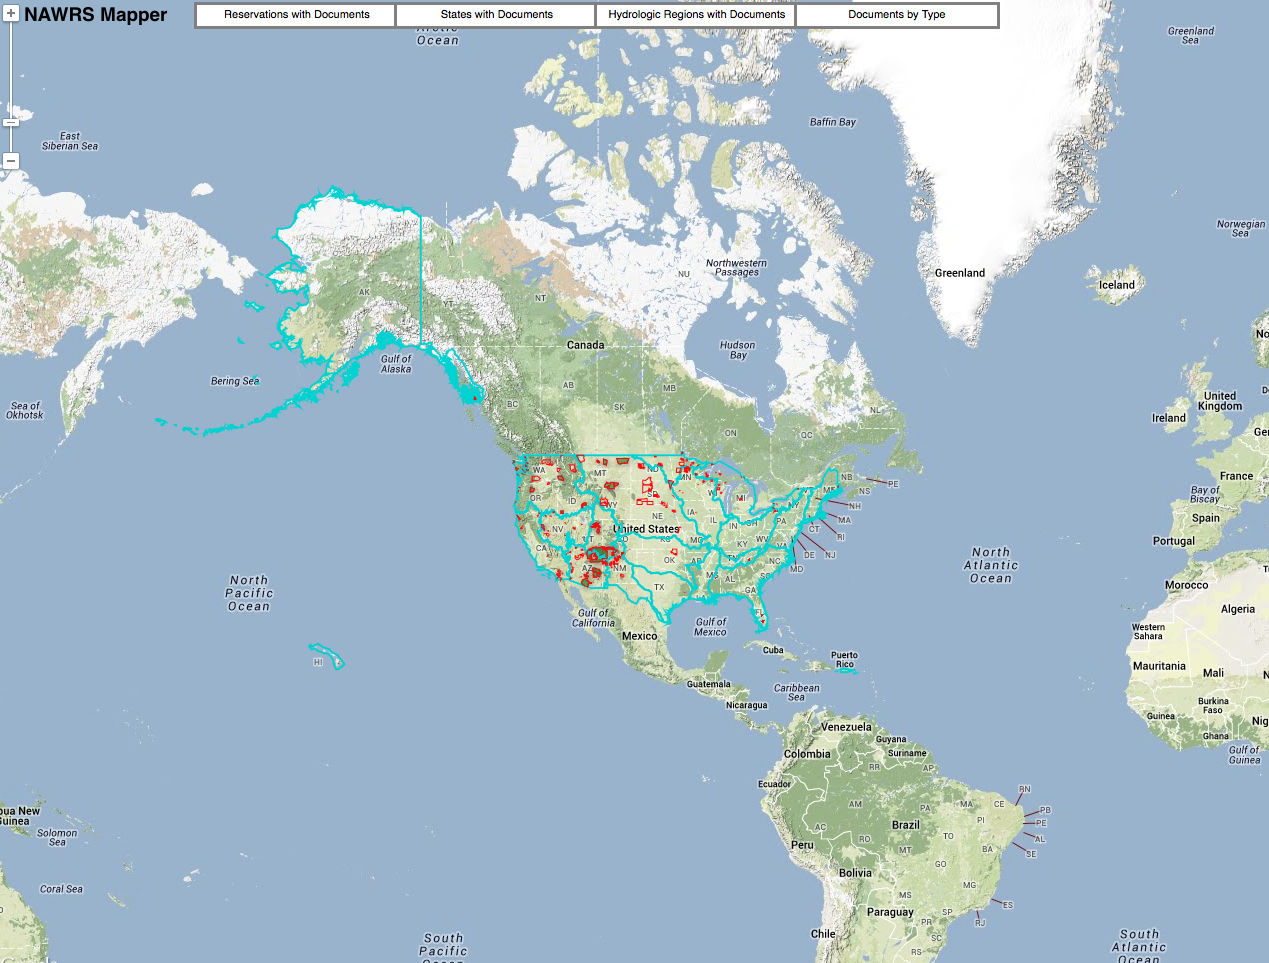
\includegraphics{images/nawrs.jpg}~

\url{http://karlbenedict.com/nawrs/}

Fusion Tables: \href{http://tinyurl.com/npx2q6g}{Merged document info},
\href{http://tinyurl.com/qyy4kew}{State bounding boxes},
\href{http://tinyurl.com/or5xuxc}{HUC bounding boxes}

\hyperdef{}{complexMap}{\label{complexMap}}
\begin{Shaded}
\begin{Highlighting}[numbers=left,,]
\DataTypeTok{<!DOCTYPE }\NormalTok{html}\DataTypeTok{>}
\KeywordTok{<html>}
\KeywordTok{<head>}
\KeywordTok{<link}\OtherTok{ rel=}\StringTok{"stylesheet"}\OtherTok{ type=}\StringTok{"text/css"}\OtherTok{ href=}\StringTok{"styles.css"}\KeywordTok{>}

\KeywordTok{<script}\OtherTok{ type=}\StringTok{"text/javascript"} 
\OtherTok{    src=}\StringTok{"http://maps.google.com/maps/api/js?v=3.2}\ErrorTok{&}\StringTok{sensor=false"}\KeywordTok{></script>}
\KeywordTok{<script}\OtherTok{ type=}\StringTok{"text/javascript"} 
\OtherTok{    src=}\StringTok{"//ajax.googleapis.com/ajax/libs/jquery/1.10.1/jquery.min.js"}\KeywordTok{></script>}
\KeywordTok{<script}\OtherTok{ type=}\StringTok{"text/javascript"}\OtherTok{ src=}\StringTok{"http://www.google.com/jsapi"}\KeywordTok{></script>}
\KeywordTok{<script}\OtherTok{ type=}\StringTok{"text/javascript"}\OtherTok{ charset=}\StringTok{"utf-8"}\OtherTok{ src=}\StringTok{"./core.js"}\KeywordTok{></script>}

\CommentTok{<!-- DataTables and DataTables CSS -->}
\KeywordTok{<link}\OtherTok{ rel=}\StringTok{"stylesheet"}\OtherTok{ type=}\StringTok{"text/css"} 
\OtherTok{  href=}\StringTok{"http://kkb-projects.s3.amazonaws.com/nawrs/js/DataTables-1.9.4/}
\StringTok{  media/css/jquery.dataTables.css"}\KeywordTok{>}
\KeywordTok{<link}\OtherTok{ rel=}\StringTok{"stylesheet"}\OtherTok{ type=}\StringTok{"text/css"} 
\OtherTok{  href=}\StringTok{"http://kkb-projects.s3.amazonaws.com/nawrs/js/DataTables-1.9.4/extras/TableTools/}
\StringTok{  media/css/TableTools.css"}\KeywordTok{>}
\KeywordTok{<script}\OtherTok{ type=}\StringTok{"text/javascript"}\OtherTok{ charset=}\StringTok{"utf8"} 
\OtherTok{  src=}\StringTok{"http://kkb-projects.s3.amazonaws.com/nawrs/js/DataTables-1.9.4/media/js/}
\StringTok{  jquery.dataTables.min.js"}\KeywordTok{></script>}
\KeywordTok{<script}\OtherTok{ type=}\StringTok{"text/javascript"}\OtherTok{ charset=}\StringTok{"utf8"} 
\OtherTok{  src=}\StringTok{"http://kkb-projects.s3.amazonaws.com/nawrs/js/DataTables-1.9.4/extras/TableTools/media/js/}
\StringTok{  TableTools.min.js"}\KeywordTok{></script>}

\KeywordTok{</head>}

\KeywordTok{<body}\OtherTok{ onload=}\StringTok{"initialize()"}\KeywordTok{>}
  \KeywordTok{<h1>}\NormalTok{NAWRS Mapper}\KeywordTok{</h1>}
  \KeywordTok{<div}\OtherTok{ id=}\StringTok{"docsReservations"}\KeywordTok{>}\NormalTok{Reservations with Documents}\KeywordTok{</div>}
  \KeywordTok{<div}\OtherTok{ id=}\StringTok{"docsReservationsPopUp"}\KeywordTok{><ul}\OtherTok{ id=}\StringTok{"docsReservationsList"}\KeywordTok{></ul></div>}
  \KeywordTok{<div}\OtherTok{ id=}\StringTok{"docsStates"}\KeywordTok{>}\NormalTok{States with Documents}\KeywordTok{</div>}
  \KeywordTok{<div}\OtherTok{ id=}\StringTok{"docsStatesPopUp"}\KeywordTok{><ul}\OtherTok{ id=}\StringTok{"docsStatesList"}\KeywordTok{></ul></div>}
  \KeywordTok{<div}\OtherTok{ id=}\StringTok{"docsHucs"}\KeywordTok{>}\NormalTok{Hydrologic Regions with Documents}\KeywordTok{</div>}
  \KeywordTok{<div}\OtherTok{ id=}\StringTok{"docsHucsPopUp"}\KeywordTok{><ul}\OtherTok{ id=}\StringTok{"docsHucsList"}\KeywordTok{></ul></div>}
  \KeywordTok{<div}\OtherTok{ id=}\StringTok{"docsType"}\KeywordTok{>}\NormalTok{Documents by Type}\KeywordTok{</div>}
  \KeywordTok{<div}\OtherTok{ id=}\StringTok{"docsTypePopUp"}\KeywordTok{><ul}\OtherTok{ id=}\StringTok{"docsTypeList"}\KeywordTok{></ul></div>}
  \KeywordTok{<div}\OtherTok{ id=}\StringTok{"map_canvas"}\KeywordTok{></div>}
  \KeywordTok{<div}\OtherTok{ id=}\StringTok{"docListHandle"}\KeywordTok{>}\NormalTok{Document List}\KeywordTok{</div>}
  \KeywordTok{<div}\OtherTok{ id=}\StringTok{"docList"}\KeywordTok{>}
    \KeywordTok{<table}\OtherTok{ id=}\StringTok{"docListTable"}\KeywordTok{>}
  \KeywordTok{</table>}
  \KeywordTok{</div>}
  
\KeywordTok{</body>}

\KeywordTok{</html>}
\end{Highlighting}
\end{Shaded}

\section{OpenLayers Javascript
Framework}\label{openlayers-javascript-framework}

\subsubsection{Outline}\label{outline-1}

\begin{itemize}
\item
  Capabilities
\item
  OpenLayers = Javascript (by example)
\end{itemize}

\subsubsection{OpenLayers Capabilities}\label{openlayers-capabilities}

\begin{itemize}
\itemsep1pt\parskip0pt\parsep0pt
\item
  Support for Multiple basemaps: \emph{Google}, \emph{Yahoo},
  \emph{Bing}, \emph{OpenStreetMap}
\item
  Model for interaction with multiple map server platforms:
  \emph{ArcGIS} (REST \& cache), \emph{ArcIMS}, \emph{KaMap},
  \emph{MapServer}
\item
  Support for key OGC standards: \emph{WMS}, \emph{WMTS}, \emph{WFS},
  \emph{GML}, \emph{KML}, \emph{SLD}
\item
  Multiple control types: \emph{Navigation}, \emph{Pan}, \emph{Zoom},
  \emph{Overview}, \emph{Scale}, \emph{Feature Creation \& Editing},
  \emph{Graticle}, \emph{Layer Switcher}
\item
  Custom styled features with associated attributes: \emph{Curve},
  \emph{LinearRing}, \emph{LineString}, \emph{MultiLineString},
  \emph{MultiPoint}, \emph{MultiPolygon}, \emph{Point}, \emph{Polygon},
  \emph{Rectangle}
\item
  Support for many formats for data read and write: \emph{ArcXML},
  \emph{ATOM}, \emph{GeoRSS}, \emph{GPX}, \emph{KML}, \emph{WKT}, any
  many others
\item
  Open Source, enabling modification and integration into other systems
  (e.g. \href{http://geoext.org/}{GeoExt})
\end{itemize}

\subsubsection{Distinguishing Characteristics Between OpenLayers and
Google
Maps}\label{distinguishing-characteristics-between-openlayers-and-google-maps}

\begin{itemize}
\itemsep1pt\parskip0pt\parsep0pt
\item
  Greater emphasis on client-side processing - Client access and
  rendering of data files that Google's servers otherwise take care of
  (pros \& cons to this approach)
\item
  Integrated support for OGC services and their products
\item
  Support for different projections (adds complexity)
\item
  API more rich in options ==\textgreater{} more complexity
\end{itemize}

\subsubsection{Resources}\label{resources}

\href{http://openlayers.org/}{OpenLayers Home Page}

\href{http://dev.openlayers.org/apidocs/files/OpenLayers-js.html}{Application
Programming Interface (API) Reference}

\href{http://openlayers.org/dev/examples/}{Examples}

\subsubsection{Demonstrations and
Examples}\label{demonstrations-and-examples}

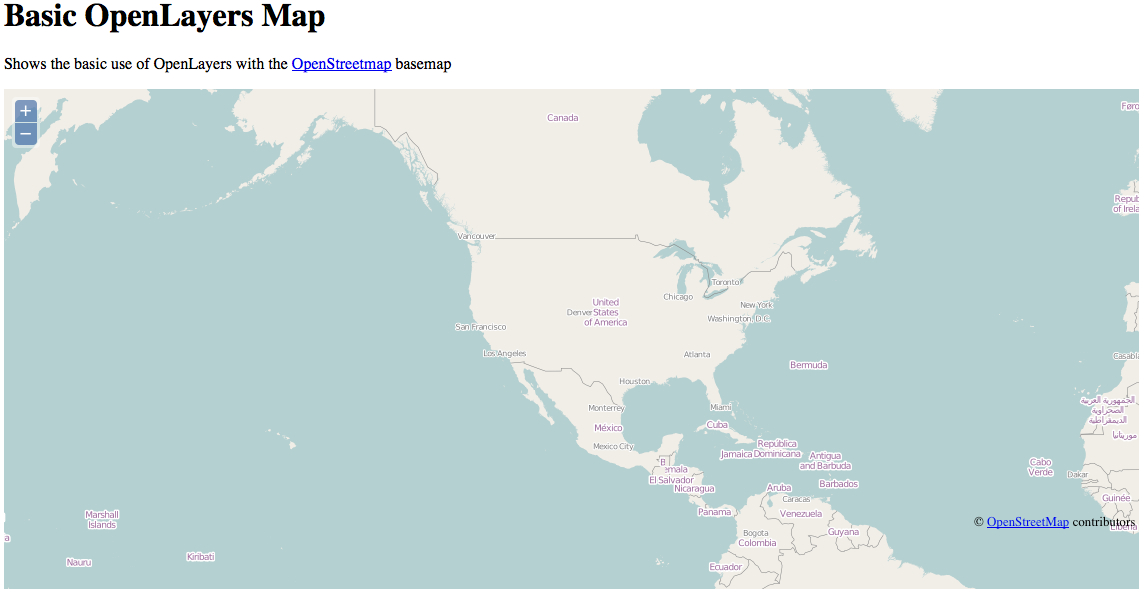
\includegraphics{images/OpenLayers_01.jpg}~

\begin{itemize}
\itemsep1pt\parskip0pt\parsep0pt
\item
  \href{http://karlbenedict.com/presentations/2014-04-NMGIC/examples/openLayers01_osm.html}{Basic
  Mapper} (with OpenStreetMaps {[}OSM{]} base map)
\end{itemize}

\hyperdef{}{OpenLayersux5f01ux5fdemo}{\label{OpenLayersux5f01ux5fdemo}}
\begin{Shaded}
\begin{Highlighting}[numbers=left,,]
\KeywordTok{<html}\OtherTok{ xmlns=}\StringTok{"http://www.w3.org/1999/xhtml"}\KeywordTok{>}
  \KeywordTok{<head>}
    \KeywordTok{<script}\OtherTok{ type=}\StringTok{"text/javascript"}\OtherTok{ src=}\StringTok{"http://openlayers.org/api/OpenLayers.js"}\KeywordTok{></script>}
    \KeywordTok{<script}\OtherTok{ type=}\StringTok{"text/javascript"}\KeywordTok{>}        
        \CommentTok{// define global variables}
        \KeywordTok{var} \NormalTok{lon = -}\FloatTok{106.5}\NormalTok{;}
        \KeywordTok{var} \NormalTok{lat = }\DecValTok{36}\NormalTok{;}
        \KeywordTok{var} \NormalTok{zoom = }\DecValTok{3}\NormalTok{;}
        \KeywordTok{var} \NormalTok{map;}
        \KeywordTok{var} \NormalTok{layer;}

        \CommentTok{// =============== Initialization function ===================}
\ErrorTok{        function init()\{}
\ErrorTok{            map = new OpenLayers.Map( 'map' );}
            
            \CommentTok{// =========== OSM Map ====================}
\ErrorTok{            layer = new OpenLayers.Layer.OSM( "Open Street Map");}
\ErrorTok{            map.addLayer(layer);}
            
\ErrorTok{            map.setCenter(}
\ErrorTok{                new OpenLayers.LonLat(lon, lat).transform(}
\ErrorTok{                    new OpenLayers.Projection("EPSG:4326"),}
\ErrorTok{                    map.getProjectionObject()}
                \NormalTok{), zoom}
            \NormalTok{);                }
        \NormalTok{\}}
        \CommentTok{// =============== End of Initialization Function ============}
        
    \KeywordTok{</script>}
    \KeywordTok{<style}\OtherTok{ type=}\StringTok{"text/css"}\KeywordTok{>}
        \FloatTok{#map} \KeywordTok{\{width:}\DataTypeTok{90%}\KeywordTok{;} \KeywordTok{height:}\DataTypeTok{500px}\KeywordTok{\}}
    \KeywordTok{</style>}
  \KeywordTok{</head>}
  \KeywordTok{<body}\OtherTok{ onload=}\StringTok{"init()"}\KeywordTok{>}
    \KeywordTok{<h1>}\NormalTok{Basic OpenLayers Map}\KeywordTok{</h1>}
    \KeywordTok{<p>}\NormalTok{Shows the basic use of OpenLayers with the }
    \KeywordTok{<a}\OtherTok{ href=}\StringTok{"http://www.openstreetmap.org/"}\KeywordTok{>}\NormalTok{OpenStreetmap}\KeywordTok{</a>} \NormalTok{basemap}\KeywordTok{</p>}   
    \CommentTok{<!-- Map DIV -->}
    \KeywordTok{<div}\OtherTok{ id=}\StringTok{"map"}\KeywordTok{></div>}    
  \KeywordTok{</body>}
\KeywordTok{</html>}
\end{Highlighting}
\end{Shaded}

\subsubsection{Demonstration and Examples - Online
Resources}\label{demonstration-and-examples---online-resources}

\begin{itemize}
\itemsep1pt\parskip0pt\parsep0pt
\item
  \href{http://karlbenedict.com/presentations/2014-04-NMGIC/examples/openLayers02_proprietary.html}{Mapper}
  with a variety of base maps (Google, Bing, Yahoo, OSM)
\item
  Basic Mapper with Controls:
  \href{http://karlbenedict.com/presentations/2014-04-NMGIC/examples/openLayers03_none.html}{No
  Controls},
  \href{http://karlbenedict.com/presentations/2014-04-NMGIC/examples/openLayers03_layerSwitcher.html}{Layer
  Switcher},
  \href{http://karlbenedict.com/presentations/2014-04-NMGIC/examples/openLayers03_controlArray.html}{Control
  Array},
  \href{http://karlbenedict.com/presentations/2014-04-NMGIC/examples/openLayers03_Overlay.html}{Overlay
  Map},
  \href{http://karlbenedict.com/presentations/2014-04-NMGIC/examples/openLayers03_Scale.html}{Scale
  Information}
\item
  Positioning Controls with the \texttt{moveTo} function:
  \href{http://karlbenedict.com/presentations/2014-04-NMGIC/examples/openLayers04_MovedControls.html}{two
  controls moved}
\end{itemize}

\subsubsection{Map Object Options}\label{map-object-options}

Map Object Options
\href{http://dev.openlayers.org/releases/OpenLayers-2.13/doc/apidocs/files/OpenLayers/Map-js.html}{API
Reference}

Two methods for constructing a new \texttt{OpenLayers.Map} object

\hyperdef{}{OpenLayersux5f02ux5fMapux5foptions}{\label{OpenLayersux5f02ux5fMapux5foptions}}
\begin{Shaded}
\begin{Highlighting}[numbers=left,,]
    \NormalTok{// create a map with default options in an element with the id "map1"}
    \NormalTok{var map = new OpenLayers.Map("map1");}
    
    \NormalTok{// create a map with non-default options in an element with id "map2"}
    \NormalTok{var options = \{}
        \NormalTok{maxExtent: new OpenLayers.Bounds(-200000, -200000, 200000, 200000),}
        \NormalTok{maxResolution: 156543,}
        \NormalTok{units: 'm',}
        \NormalTok{projection: "EPSG:41001"}
    \NormalTok{\};}
    \NormalTok{var map = new OpenLayers.Map("map2", options);}
    
    \NormalTok{// map with non-default options - same as above but with a single argument}
    \NormalTok{var map = new OpenLayers.Map(\{}
        \NormalTok{div: "map_id",}
        \NormalTok{maxExtent: new OpenLayers.Bounds(-200000, -200000, 200000, 200000),}
        \NormalTok{maxResolution: 156543,}
        \NormalTok{units: 'm',}
        \NormalTok{projection: "EPSG:41001"}
    \NormalTok{\});}
\end{Highlighting}
\end{Shaded}

Excerpts from the API documentation

\begin{description}
\item[\texttt{allOverlays}]
\{Boolean\} Allow the map to function with ``overlays'' only. Defaults
to false. If true, the lowest layer in the draw order will act as the
base layer. In addition, if set to true, all layers will have
isBaseLayer set to false when they are added to the map.
\item[\texttt{div}]
\{DOMElement\textbar{}String\} The element that contains the map (or an
id for that element). If the OpenLayers.Map constructor is called with
two arguments, this should be provided as the first argument.
Alternatively, the map constructor can be called with the options object
as the only argument. In this case (one argument), a div property may or
may not be provided. If the div property is not provided, the map can be
rendered to a container later using the render method.
\item[\texttt{layers}]
\{Array(OpenLayers.Layer)\} Ordered list of layers in the map
\item[\texttt{tileSize}]
\{OpenLayers.Size\} Set in the map options to override the default tile
size for this map.
\item[\texttt{projection}]
\{String\} Set in the map options to override the default projection
string this map - also set \texttt{maxExtent}, \texttt{maxResolution},
and \texttt{units} if appropriate. Default is ``EPSG:4326''.
\item[\texttt{units}]
\{String\} The map units. Defaults to `degrees'. Possible values are
`degrees' (or `dd'), `m', `ft', `km', `mi', `inches'.
\item[\texttt{resolutions}]
\{Array(Float)\} A list of map resolutions (map units per pixel) in
descending order. If this is not set in the layer constructor, it will
be set based on other resolution related properties (maxExtent,
maxResolution, maxScale, etc.).
\item[\texttt{maxResolution}]
\{Float\} Default max is 360 deg / 256 px, which corresponds to zoom
level 0 on gmaps. Specify a different value in the map options if you
are not using a geographic projection and displaying the whole world.
\item[\texttt{minResolution}]
\{Float\}
\item[\texttt{maxScale}]
\{Float\}
\item[\texttt{minScale}]
\{Float\}
\item[\texttt{maxExtent}]
\{OpenLayers.Bounds\} The maximum extent for the map. Defaults to the
whole world in decimal degrees (-180, -90, 180, 90). Specify a different
extent in the map options if you are not using a geographic projection
and displaying the whole world.
\item[\texttt{minExtent}]
\{OpenLayers.Bounds\}
\item[\texttt{restrictedExtent}]
\{OpenLayers.Bounds\} Limit map navigation to this extent where
possible. If a non-null restrictedExtent is set, panning will be
restricted to the given bounds. In addition, zooming to a resolution
that displays more than the restricted extent will center the map on the
restricted extent. If you wish to limit the zoom level or resolution,
use maxResolution.
\item[\texttt{numZoomLevels}]
\{Integer\} Number of zoom levels for the map. Defaults to 16. Set a
different value in the map options if needed.
\end{description}

\subsubsection{Layer Object Options}\label{layer-object-options}

Layer Object Options
\href{http://dev.openlayers.org/releases/OpenLayers-2.13/doc/apidocs/files/OpenLayers/Layer-js.html}{API
Reference}

Common Pattern of Layer Object Creation (varies some depending upon the
specific layer type)

\hyperdef{}{OpenLayersux5f02ux5fLayerux5foptions}{\label{OpenLayersux5f02ux5fLayerux5foptions}}
\begin{Shaded}
\begin{Highlighting}[numbers=left,,]
    \NormalTok{new OpenLayers.Layer.*** (}
        \NormalTok{'layer name',}
        \NormalTok{'layer URL',}
        \NormalTok{\{server-related options\}, }
        \NormalTok{\{OpenLayers Layer Object options\}}
    \NormalTok{)}
\end{Highlighting}
\end{Shaded}

\begin{description}
\item[\texttt{id}]
\{String\}
\item[\texttt{name}]
\{String\}
\item[\texttt{isBaseLayer}]
\{Boolean\} Whether or not the layer is a base layer. This should be set
individually by all subclasses. Default is false
\item[\texttt{displayInLayerSwitcher}]
\{Boolean\} Display the layer's name in the layer switcher. Default is
true.
\item[\texttt{visibility}]
\{Boolean\} The layer should be displayed in the map. Default is true.
\item[\texttt{attribution}]
\{String\} Attribution string, displayed when an
OpenLayers.Control.Attribution has been added to the map.
\item[\texttt{projection}]
\{OpenLayers.Projection\} or \{String\} Set in the layer options to
override the default projection string this layer - also set maxExtent,
maxResolution, and units if appropriate. Can be either a string or an
OpenLayers.Projection object when created -- will be converted to an
object when setMap is called if a string is passed.
\item[\texttt{units}]
\{String\} The layer map units. Defaults to `degrees'. Possible values
are `degrees'' (or `dd'), `m', `ft', `km', `mi', `inches'.
\item[\texttt{scales}]
\{Array\} An array of map scales in descending order. The values in the
array correspond to the map scale denominator. Note that these values
only make sense if the display (monitor) resolution of the client is
correctly guessed by whomever is configuring the application. In
addition, the units property must also be set. Use resolutions instead
wherever possible.
\item[\texttt{resolutions}]
\{Array\} A list of map resolutions (map units per pixel) in descending
order. If this is not set in the layer constructor, it will be set based
on other resolution related properties (maxExtent, maxResolution,
maxScale, etc.).
\item[\texttt{maxExtent}]
\{OpenLayers.Bounds\} The center of these bounds will not stray outside
of the viewport extent during panning. In addition, if
displayOutsideMaxExtent is set to false, data will not be requested that
falls completely outside of these bounds.
\item[\texttt{minExtent}]
\{OpenLayers.Bounds\}
\item[\texttt{maxResolution}]
\{Float\} Default max is 360 deg / 256 px, which corresponds to zoom
level 0 on gmaps. Specify a different value in the layer options if you
are not using a geographic projection and displaying the whole world.
\item[\texttt{minResolution}]
\{Float\}
\item[\texttt{numZoomLevels}]
\{Integer\}
\item[\texttt{minScale}]
\{Float\}
\item[\texttt{maxScale}]
\{Float\}
\item[\texttt{displayOutsideMaxExtent}]
\{Boolean\} Request map tiles that are completely outside of the max
extent for this layer. Defaults to false.
\item[\texttt{transitionEffect}]
\{String\} The transition effect to use when the map is panned or
zoomed.
\item[There are currently two supported values]
\texttt{null} No transition effect (the default).

\texttt{resize} Existing tiles are resized on zoom to provide a visual
effect of the zoom having taken place immediately. As the new tiles
become available, they are drawn over top of the resized tiles.
\end{description}

\subsubsection{Additional Map and Layer Object Functions \&
Events}\label{additional-map-and-layer-object-functions-events}

Both Map and Layer Objects have a number of associated functions as well

\begin{itemize}
\itemsep1pt\parskip0pt\parsep0pt
\item
  Retrieving object properties programmatically with \texttt{Get}
  functions.
\item
  Modifying existing object properties with \texttt{Set} functions
\item
  Map destruction, and reconfiguration
\item
  Linkage of object events with Javascript functions
\end{itemize}

\subsubsection{WMS Layer Configuration}\label{wms-layer-configuration}

Some key issues to be aware of when using the
\href{http://dev.openlayers.org/releases/OpenLayers-2.13/doc/apidocs/files/OpenLayers/Layer/WMS-js.html}{WMS
Layer Class}:

\begin{itemize}
\itemsep1pt\parskip0pt\parsep0pt
\item
  The \emph{projection} of the map object must be supported by the
  included WMS service (review the WMS GetCapabilities response to see
  what projections are supported by the service)
\item
  The \emph{layers} parameter/property must be provided as part of the
  server-related property list (the layer names also come from the
  GetCapabilities response)
\item
  Other WMS parameters may be provided as well to ``adjust'' the request
  automatically generated by OpenLayers
\end{itemize}

Sample WMS Layer Object Creation

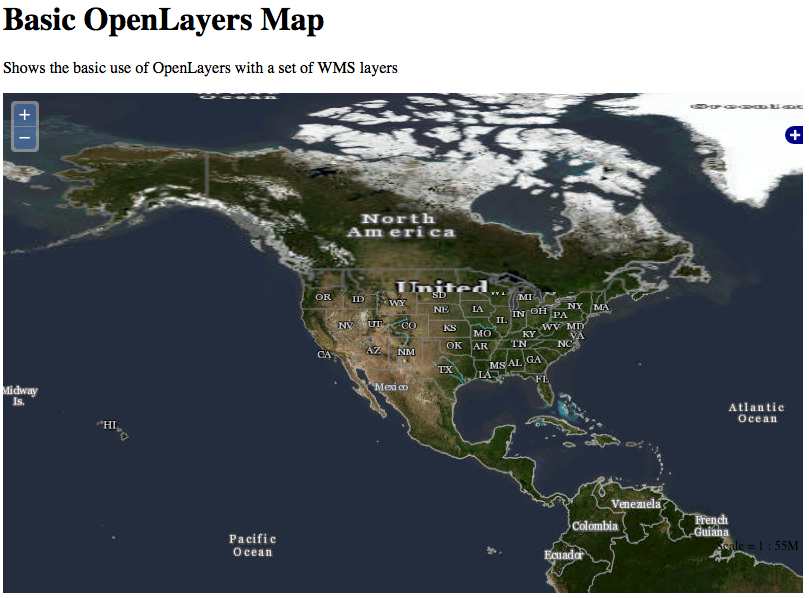
\includegraphics{images/OpenLayers_02.jpg}~

\url{http://karlbenedict.com/presentations/2014-04-NMGIC/examples/openLayers10_wms01.html}

\hyperdef{}{OpenLayersux5f02ux5fWmsLayerux5foptions}{\label{OpenLayersux5f02ux5fWmsLayerux5foptions}}
\begin{Shaded}
\begin{Highlighting}[numbers=left,,]
    \NormalTok{countiesLayer = new OpenLayers.Layer.WMS( }
        \NormalTok{"US Counties", }
        \NormalTok{"http://webservices.nationalatlas.gov/wms?",}
        \NormalTok{\{layers: "counties", version: '1.3.0', transparent: 'TRUE'\},}
        \NormalTok{\{isBaseLayer: false, visibility: false, opacity: .8\}}
    \NormalTok{);}
    \NormalTok{map.addLayer(countiesLayer);}
\end{Highlighting}
\end{Shaded}

\subsubsection{Vector Layer
Configuration}\label{vector-layer-configuration}

Vector layers support

\begin{itemize}
\itemsep1pt\parskip0pt\parsep0pt
\item
  External Data in a Variety of supported
  \href{http://dev.openlayers.org/releases/OpenLayers-2.13/doc/apidocs/files/OpenLayers/Format-js.html}{formats}
  for both \emph{reading} and \emph{writing} (just a sample):
  ArcXML.Features, GeoJSON, GeoRSS, GPX, JSON, KML, WFS, WKT
\item
  Directly encoded {[}geometries{]}{[}OpenLayers.Geometry API Link{]}:
  Collection, Curve, LinearRing, LineString, MultiLineString,
  MultiPoint, MultiPolygon, Point, Polygon, Rectangle
\item
  User created features, including support for interactive editing of
  features
\item
  \href{http://dev.openlayers.org/releases/OpenLayers-2.13/doc/apidocs/files/OpenLayers/Feature/Vector-js.html\#OpenLayers.Feature.Vector.style}{Styling}
  of Vector features
\end{itemize}

Vector Layer Objects are Typically Defined using three OpenLayers
classes

\begin{description}
\item[\texttt{Protocol}]
Connection protocol for requesting the data that would be provided from
an external source
\item[\texttt{Format}]
The OpenLayers supported format of the vector data object
\item[\texttt{Strategy}]
A specification of how OpenLayers should request the data from the
server, and also handle the data within the client (browser).
\end{description}

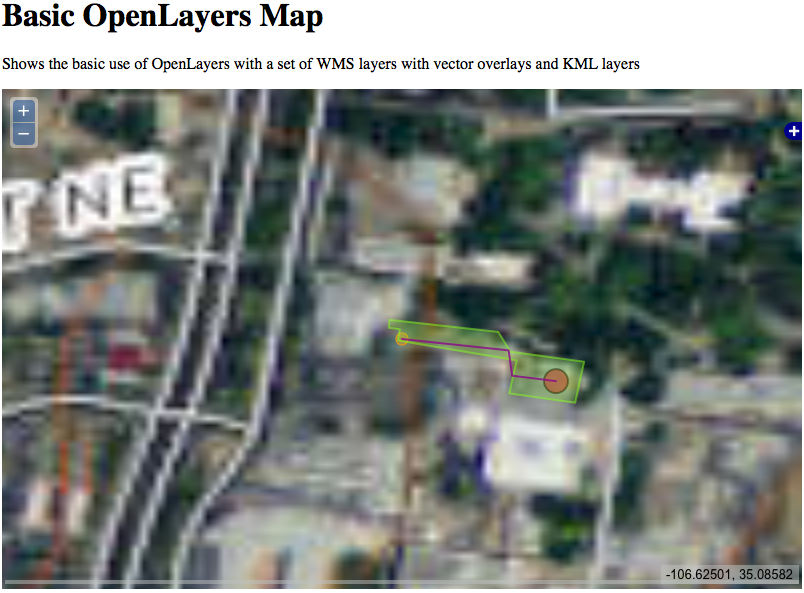
\includegraphics{images/OpenLayers_03.jpg}~

\url{http://karlbenedict.com/presentations/2014-04-NMGIC/examples/openLayers11_vectorData_KML.html}

Sample Point Feature Object creation

\hyperdef{}{OpenLayersux5f02ux5fVectorLayerux5foptions01}{\label{OpenLayersux5f02ux5fVectorLayerux5foptions01}}
\begin{Shaded}
\begin{Highlighting}[numbers=left,,]
    \NormalTok{var Coord_classroom = new OpenLayers.Geometry.Point(-106.624073,35.084280);}
    \NormalTok{var Point_classroom = new OpenLayers.Feature.Vector(Coord_classroom);}
    \NormalTok{Layers["localFeatures"].addFeatures([Point_classroom])}
\end{Highlighting}
\end{Shaded}

Sample KML Layer Object creation

\hyperdef{}{OpenLayersux5f02ux5fKMLayerux5foptions01}{\label{OpenLayersux5f02ux5fKMLayerux5foptions01}}
\begin{Shaded}
\begin{Highlighting}[numbers=left,,]
    \NormalTok{Layers.counties = new OpenLayers.Layer.Vector("KML - Counties", \{}
        \NormalTok{projection: map.displayProjection,}
        \NormalTok{strategies: [new OpenLayers.Strategy.Fixed()],}
        \NormalTok{protocol: new OpenLayers.Protocol.HTTP(\{}
            \NormalTok{url: "NMCounties.kml",}
            \NormalTok{format: new OpenLayers.Format.KML(\{}
                \NormalTok{extractAttributes: true}
            \NormalTok{\})}
        \NormalTok{\})}
    \NormalTok{\});}
    \NormalTok{map.addLayer(Layers.counties)}
\end{Highlighting}
\end{Shaded}

\section{Questions?}\label{questions}

\subsubsection{License Information}\label{license-information}

{NMGIC Spring 2014 - Google Maps \& OpenLayers Workshop} by Karl
Benedict is licensed under a Creative Commons Attribution 4.0
International License.

\end{document}
